\chapter{Results analysis}
\label{chapter:results-analysis}

In this chapter we analyse the results produced by the four models developed in this thesis. We are going to compare its results for each of the three problems considered: free Elastica, constrained Elastica and image segmentation.~\cref{tab:models-summary} summarizes the models properties.

In the image segmentation section, we compare our results with the linear model for curvature regularization of Schoenemann.

\begin{table}[H]
\centering
\begin{tabular}{r|ccccc}
Model & Implementation & Running time & Free Ela. & Constrained Ela. & Image Seg.\\
\hline
LocalSearch (LS) & medium & slow & yes(opt) & yes & no \\
FlipFlow (FF) & hard & acceptable & yes & no & yes \\
BalanceFlow (BF) & medium & acceptable & yes & no & yes \\
GraphFlow (GF) & easy & fast & yes(opt) & yes & yes
\end{tabular}
\caption{Models summary. The qualitative attributes are relative, e.g., the GraphFlow presents the lowest running time while LocalSearch presents the highest.}
\label{tab:models-summary}
\end{table}

\section{Free Elastica}

The free Elastica problem consists in to find a shape with the lowest digital Elastica. The approach to solve this problem as well the two others that follow, is to iteractively evolve a initial shape to another with lower digital Elastica value. We have ran two experiments, summarized in~\cref{tab:free-elastica-parameters-summary}, to illustrate the evolution process behaviour for each of the models described in this thesis. 

We make a distinction between the radius used to compute the balance coefficient $(bRadius)$ and the one used to estimate curvature using the II-estimator $(vRadius)$ in the validation function of GraphFlow and LocalSearch. In particular, the $vRadius$ is the one used to plot the graphs in~\cref{fig:plots-free-elastica-general,fig:plots-free-elastica-radius-choice}. Moreover, the $vRadius$ is always scaled by the grid step, while the $bRadius$ is never scaled.

\begin{table}
\centering
\begin{tabular}{|c|c|c|c|c|c|c|c|c|c|c|}
\cline{8-11}
\multicolumn{7}{c|}{} & LS & FF,BF & \multicolumn{2}{|c|}{GF}\\
\hline
Experiment & $maxIt$ & $vRadius$ & $bRadius$ & $h$ & $\alpha$ & $\beta$  & $nc$ & $m$ & $a$ & $ob$ \\
\hline
Exp-General & $400$ & $5$ & $7$ & $0.25$ & $0.01$ & $1$  & $4$ & $5$ & $2$ & $3$ \\
\hline
\multirow{2}{*}{Exp-Radius} & \multirow{2}{*}{$400$} & \multirow{2}{*}{$5$} & $7$ & \multirow{2}{*}{$0.25$} &  \multirow{2}{*}{$0.001$} & \multirow{2}{*}{$1$}  & \multirow{2}{*}{$4$} & $5$ & \multirow{2}{*}{$2$} & \multirow{2}{*}{$3$} \\
& &  & $12$ & &  & & & $10$ & &  \\
\hline
\end{tabular}
\caption{Parameter settings for the free Elastica experiments. The headers LS,FF,BF,GF identifies parameters that are exclusive for the LocalSearch, FlipFlow, BalanceFlow and GraphFlow models, respectively.}
\label{tab:free-elastica-parameters-summary}
\end{table}

\subsection{General experiment}

  The General experiment executes each model using the listed parameters in~\cref{tab:free-elastica-parameters-summary} for $5$ different parametric shapes. The results for the General experiment is shown in~\cref{fig:results-free-elastica-general}. One can check in the plots of~\cref{fig:plots-free-elastica-general} how the digital Elastica value evolves at each iteration. For this experiment we also provide~\cref{tab:rtime-free-elastica-general} with the model's respective running times.
  

We observe that both LocalSearch and GraphFlow evolves the initial shape to another closer to the optimal one, i.e., for $\alpha=0.01$, the disk of radius $10$. However, the GraphFlow model is simpler to implement and much faster than LocalSearch, as~\cref{tab:rtime-free-elastica-general} evidentiates. Even with a smaller neighborhood, the GraphFlow achieves its convergence first than LocalSearch in two ocassions, one in the square and the other in the flower evolution.

At the first iterations, FlipFlow and BalanceFlow produce shapes with lower digital Elastica energy. However, the models do not stop to evolve even if a shape of smaller perimeter and lower digital Elastica ceases to exist, and starting from this point, the digital Elastica value increases.


\begin{figure}
\center
\captionsetup{type=table}
\begin{tabular}{|l|c|c|c|c|c|}
\hline
& Pixels (initial shape) & LocalSearch & FlipFlow & BalanceFlow & GraphFlow \\
\hline
Triangle & 8315 & 4.8s/it & 0.4s/it & 0.38s/it & 0.14s/it\\
Square & 12769 & 2s/it & 0.51s/it & 0.47s/it & 0.12s/it\\
Ellipse  & 10038 & 3.1s/it & 0.64s/it & 0.57s/it & 0.1s/it \\
Flower & 26321 & 12.3s/it & 1.23s/it & 0.94s/it & 0.14s/it\\
Bean  & 25130 & 6.4s/it & 1.2s/it & 1.17s/it & 0.16s/it\\
\hline
\end{tabular}
\caption{Running time and input size of Exp-General experiment for the free Elastica.}
\label{tab:rtime-free-elastica-general} 
\end{figure}


\begin{figure}
\begin{tabular}{cccc}
LocalSearch & FlipFlow & BalanceFlow & GraphFlow\\[1em]
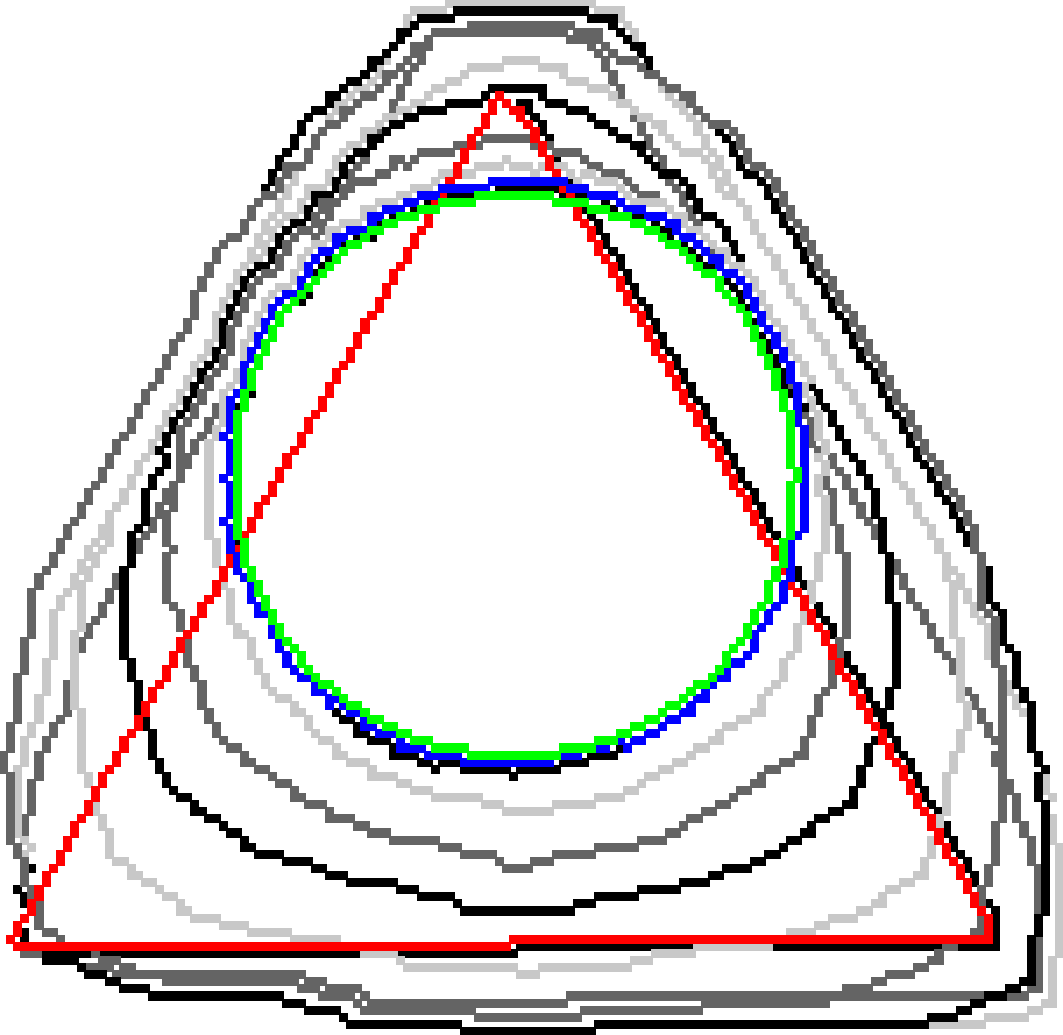
\includegraphics[scale=0.15]{figures/chapter9/free-elastica/localsearch/triangle/len_pen-0.01/radius-7/summary.pdf} & 
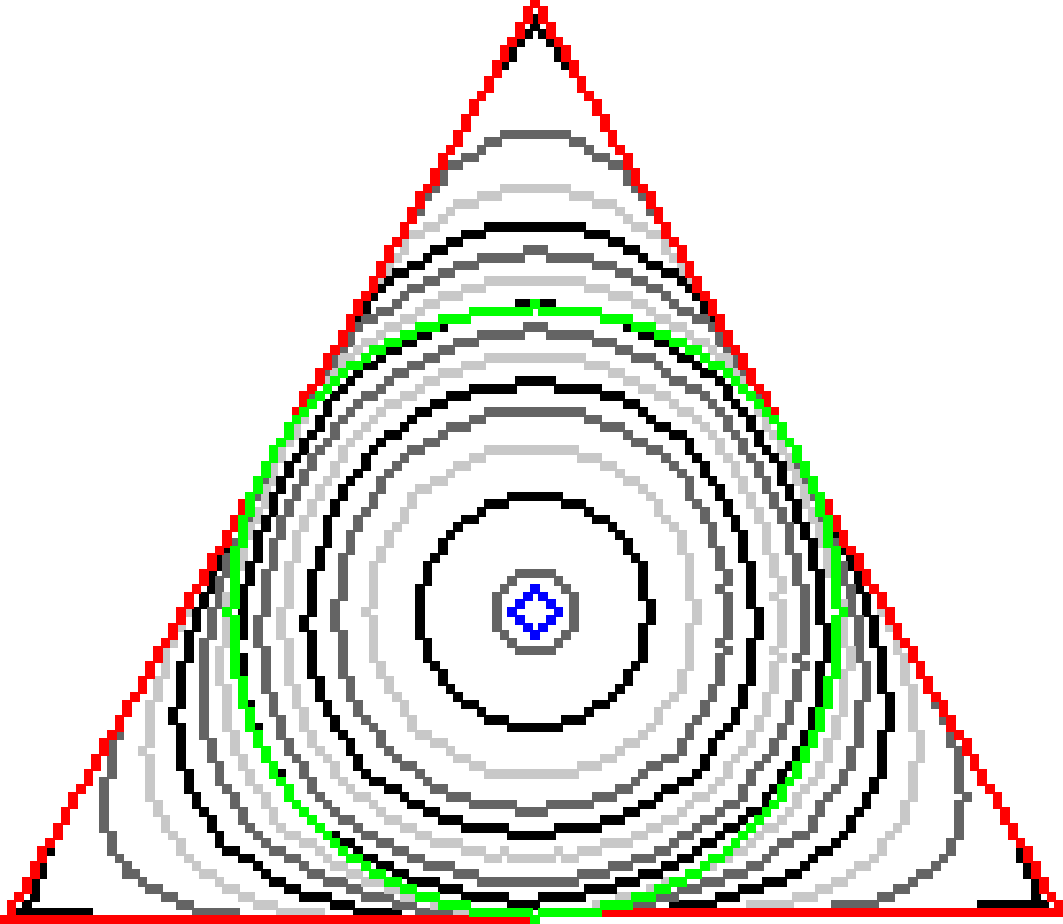
\includegraphics[scale=0.15]{figures/chapter9/free-elastica/flipflow/triangle/len_pen-0.01/radius-7/summary.pdf} &
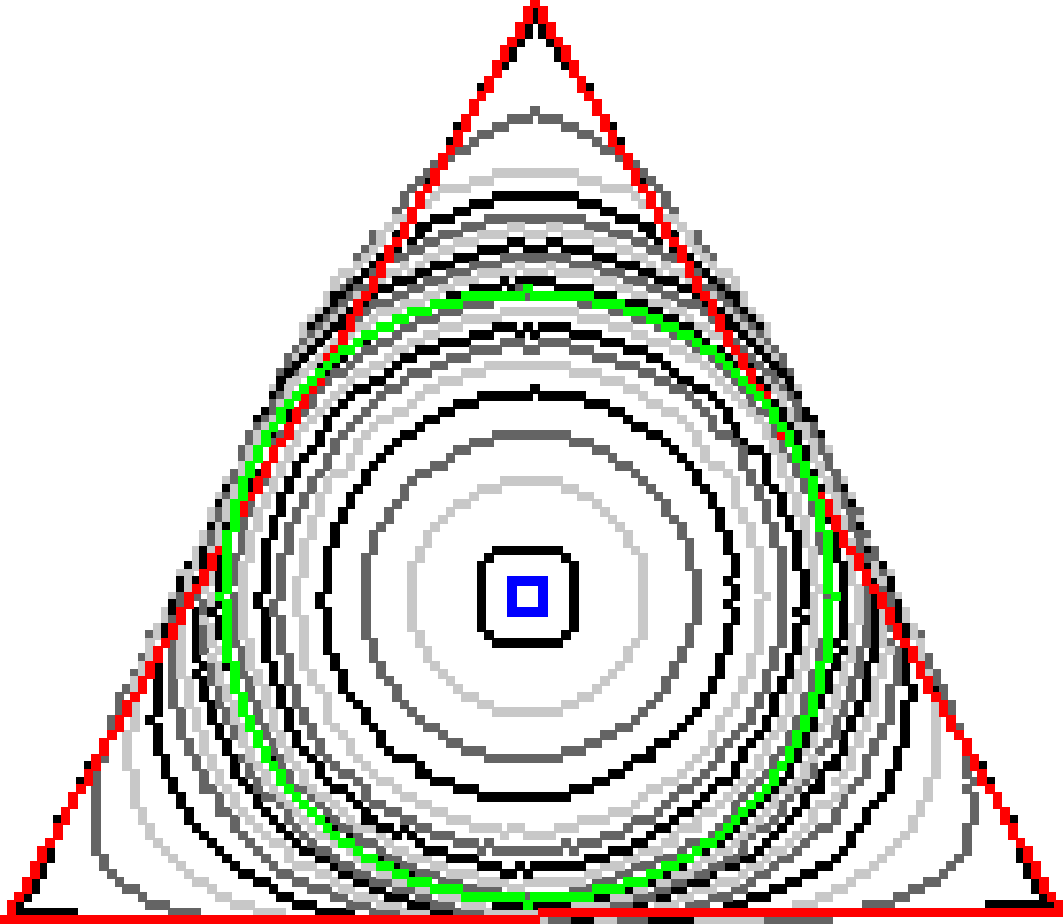
\includegraphics[scale=0.15]{figures/chapter9/free-elastica/balanceflow/triangle/len_pen-0.01/radius-7/summary.pdf} &
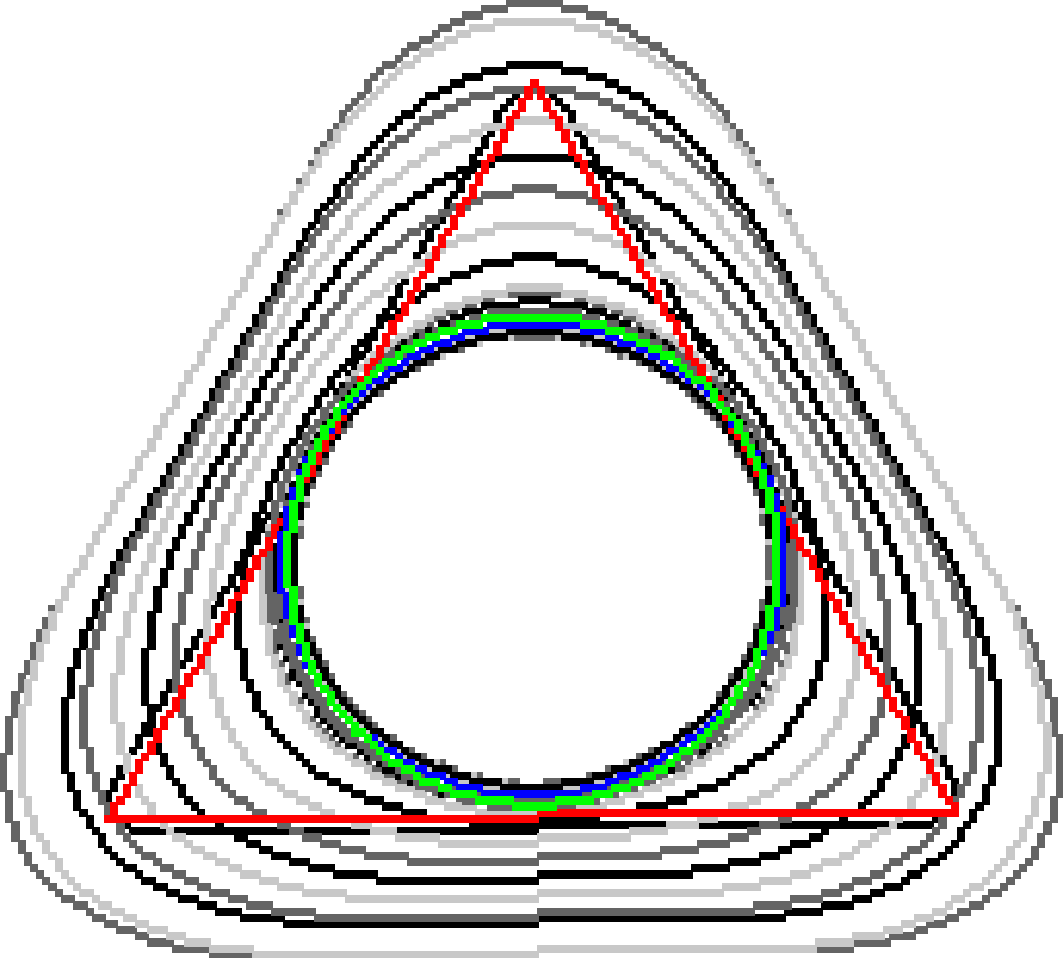
\includegraphics[scale=0.15]{figures/chapter9/free-elastica/graphflow/triangle/len_pen-0.01/radius-7/summary.pdf} \\[1em]
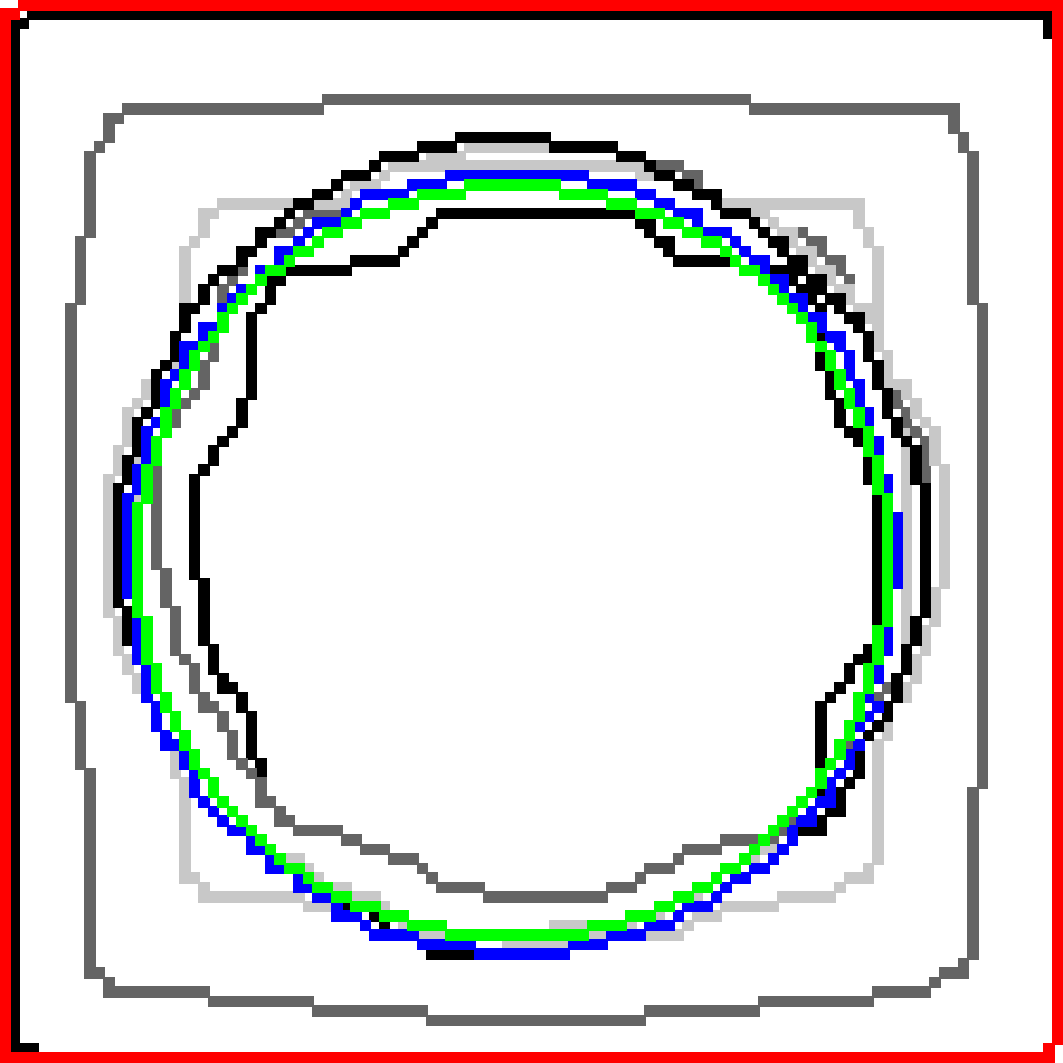
\includegraphics[scale=0.15]{figures/chapter9/free-elastica/localsearch/square/len_pen-0.01/radius-7/summary.pdf} & 
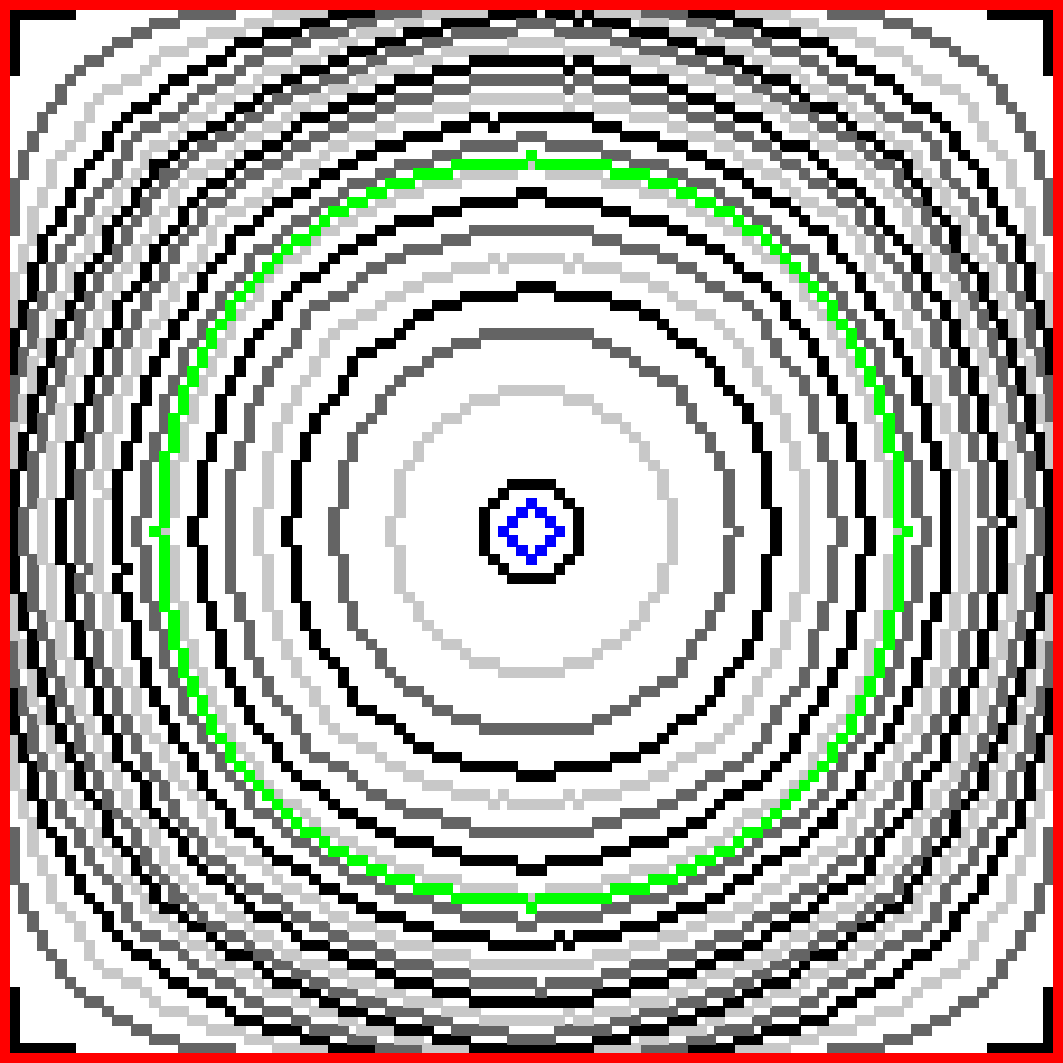
\includegraphics[scale=0.15]{figures/chapter9/free-elastica/flipflow/square/len_pen-0.01/radius-7/summary.pdf} &
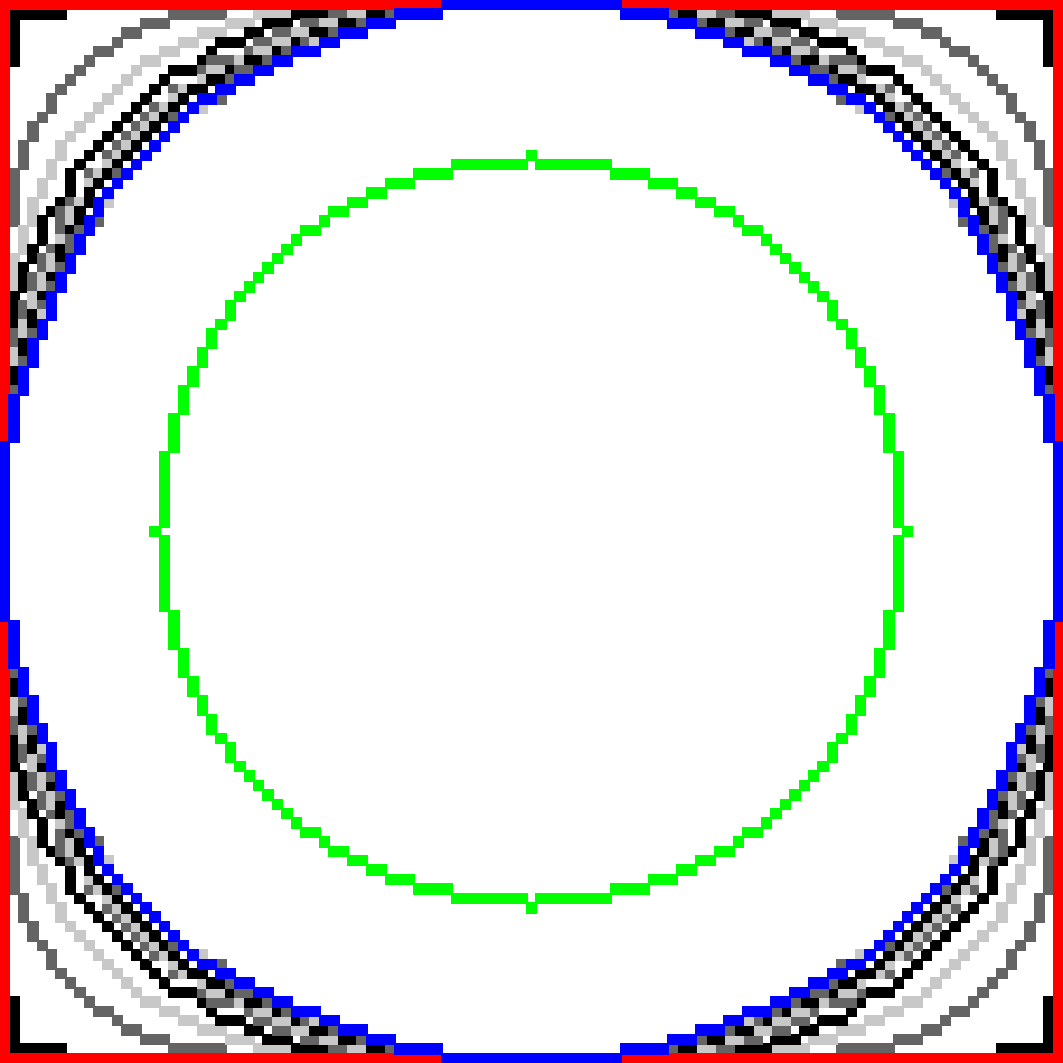
\includegraphics[scale=0.15]{figures/chapter9/free-elastica/balanceflow/square/len_pen-0.01/radius-7/summary.pdf} &
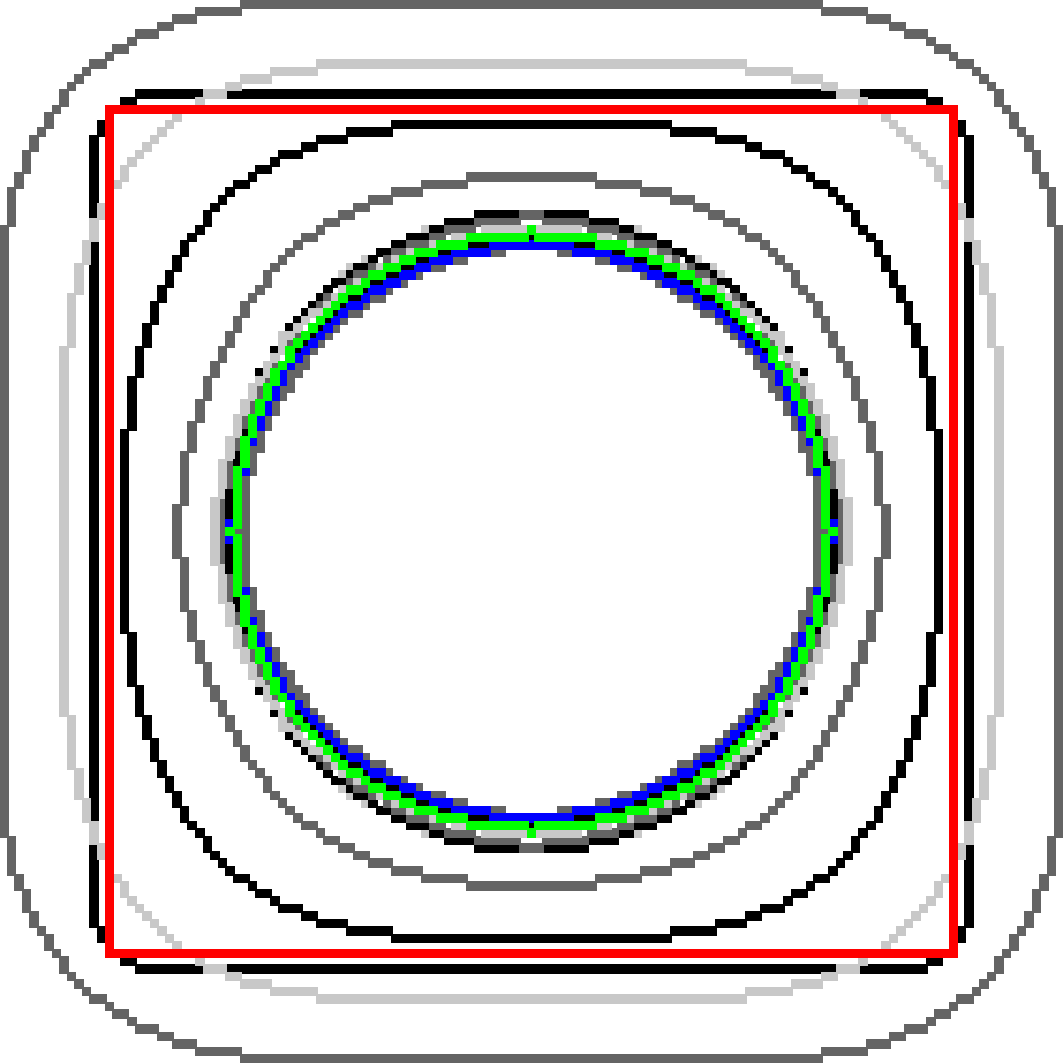
\includegraphics[scale=0.15]{figures/chapter9/free-elastica/graphflow/square/len_pen-0.01/radius-7/summary.pdf} \\[1em]
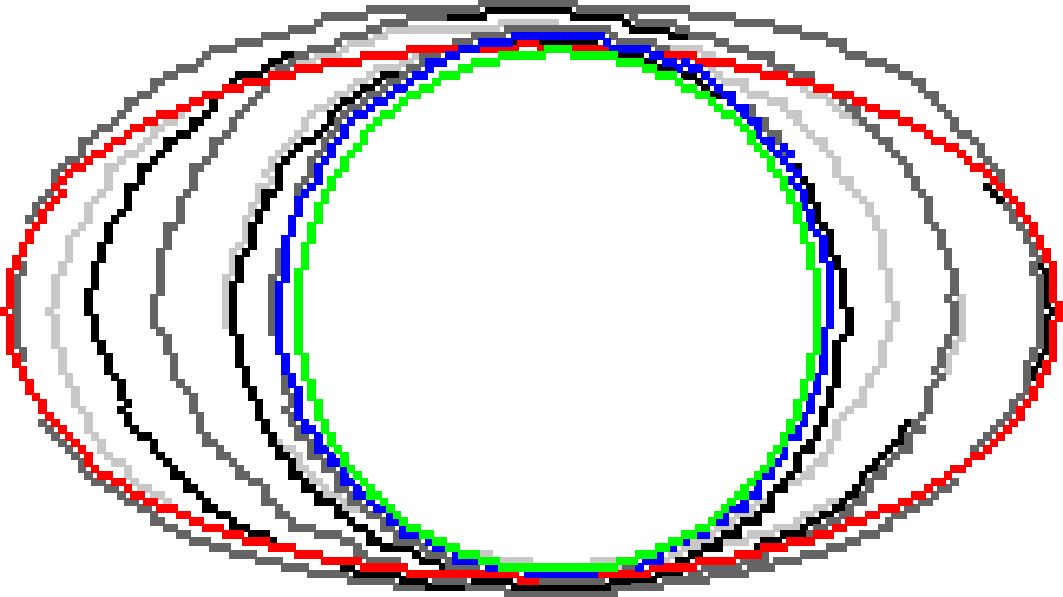
\includegraphics[scale=0.2]{figures/chapter9/free-elastica/localsearch/ellipse/len_pen-0.01/radius-7/summary.pdf} & 
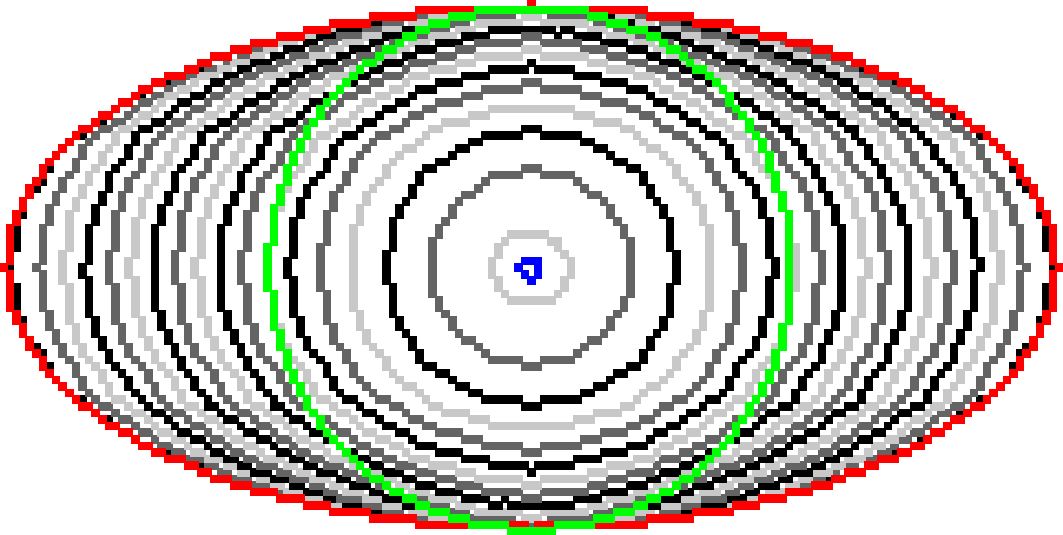
\includegraphics[scale=0.2]{figures/chapter9/free-elastica/flipflow/ellipse/len_pen-0.01/radius-7/summary.pdf} &
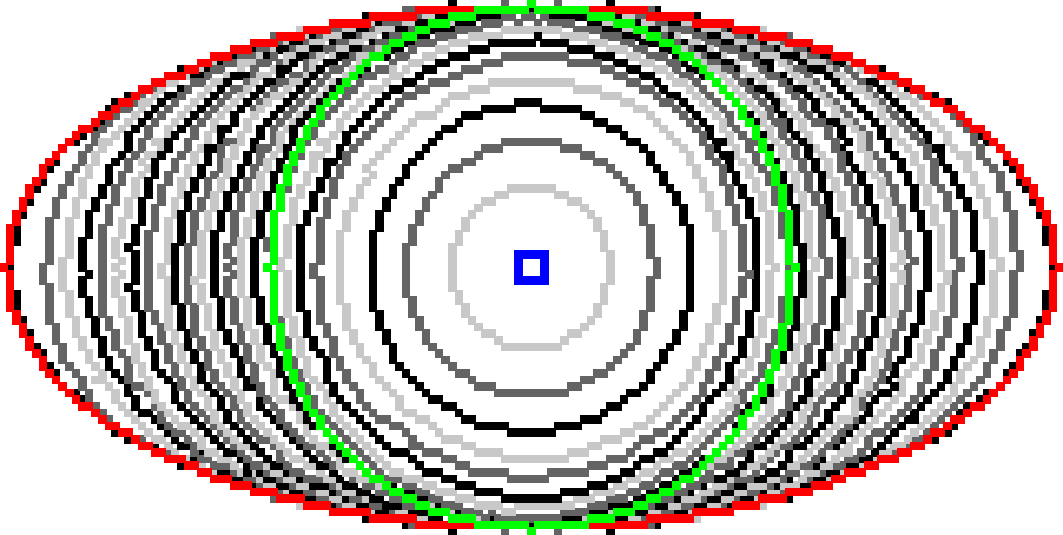
\includegraphics[scale=0.2]{figures/chapter9/free-elastica/balanceflow/ellipse/len_pen-0.01/radius-7/summary.pdf} &
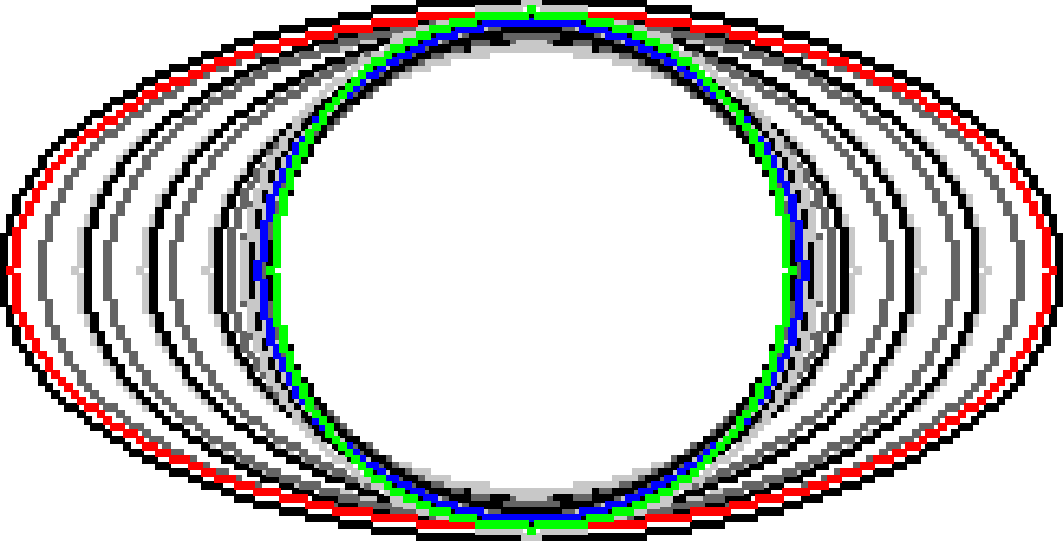
\includegraphics[scale=0.2]{figures/chapter9/free-elastica/graphflow/ellipse/len_pen-0.01/radius-7/summary.pdf} \\[1em]
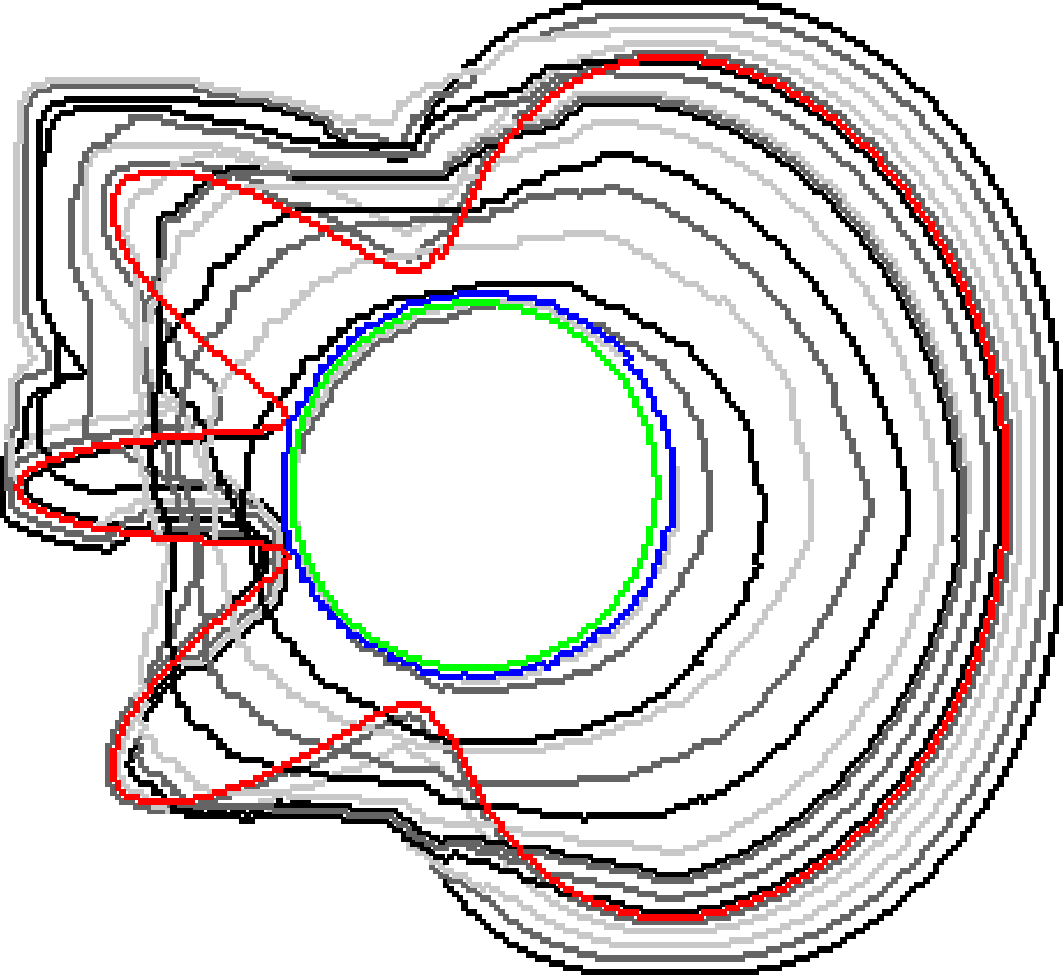
\includegraphics[scale=0.2]{figures/chapter9/free-elastica/localsearch/flower/len_pen-0.01/radius-7/summary.pdf} & 
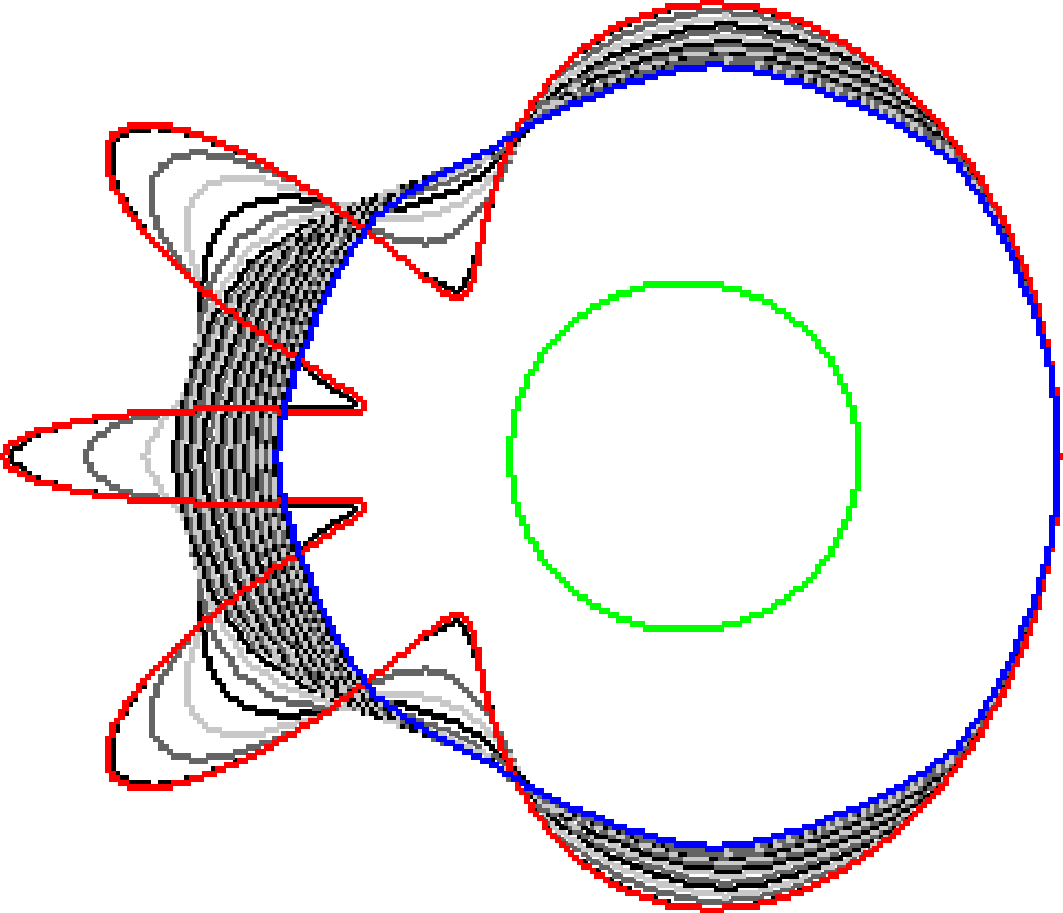
\includegraphics[scale=0.2]{figures/chapter9/free-elastica/flipflow/flower/len_pen-0.01/radius-7/summary.pdf} &
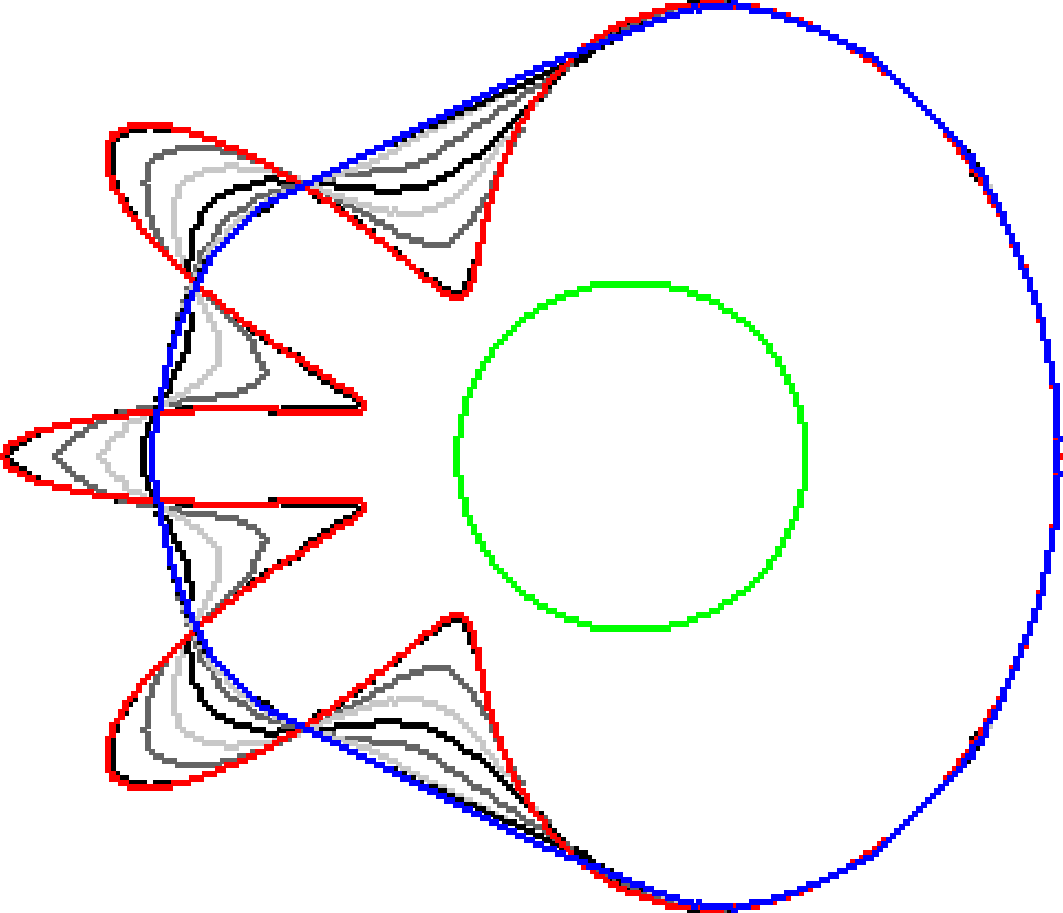
\includegraphics[scale=0.2]{figures/chapter9/free-elastica/balanceflow/flower/len_pen-0.01/radius-7/summary.pdf} &
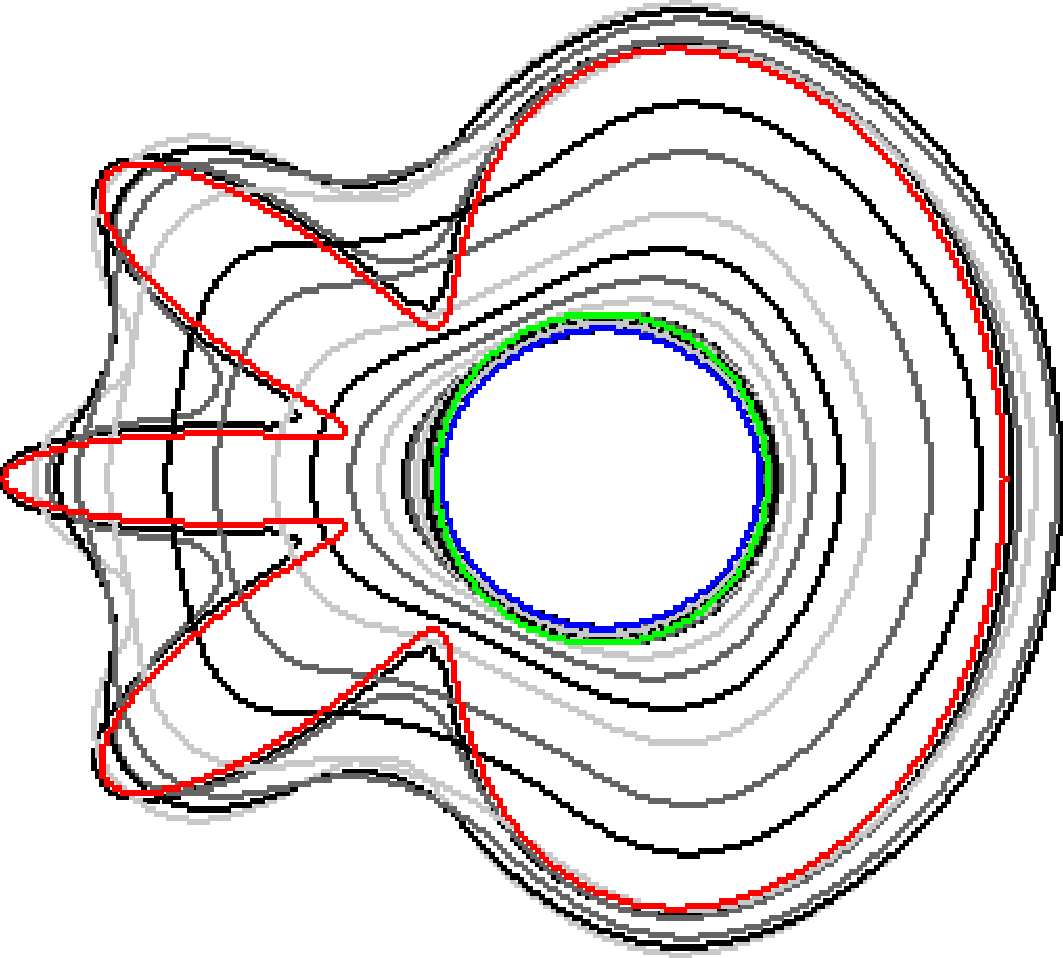
\includegraphics[scale=0.2]{figures/chapter9/free-elastica/graphflow/flower/len_pen-0.01/radius-7/summary.pdf} \\[1em]
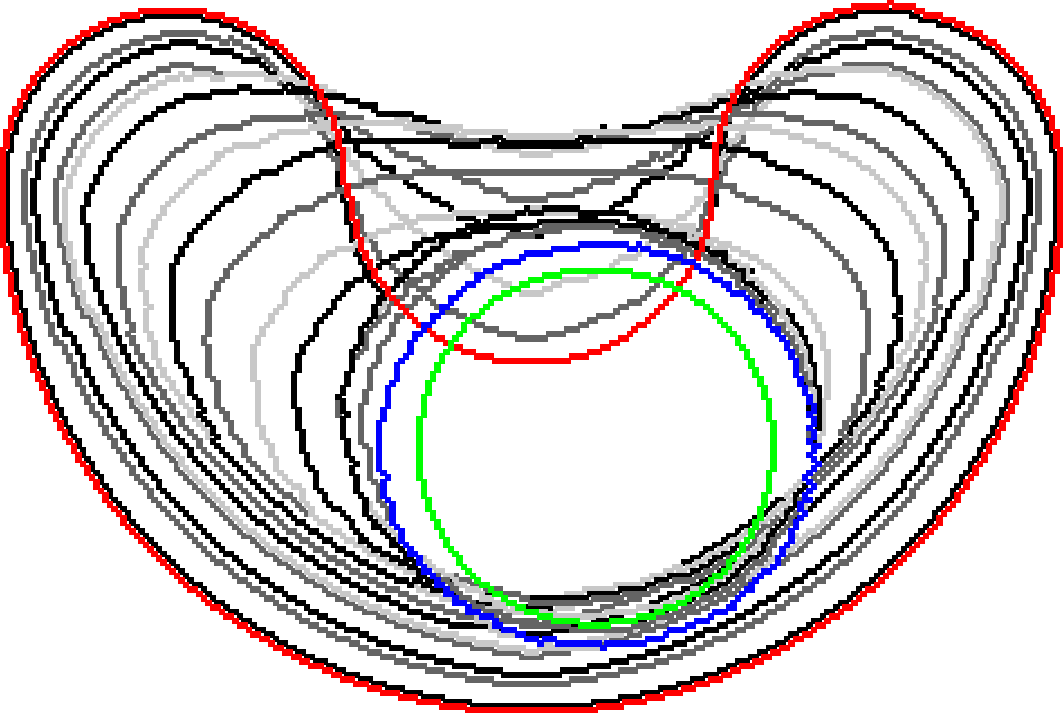
\includegraphics[scale=0.2]{figures/chapter9/free-elastica/localsearch/bean/len_pen-0.01/radius-7/summary.pdf} & 
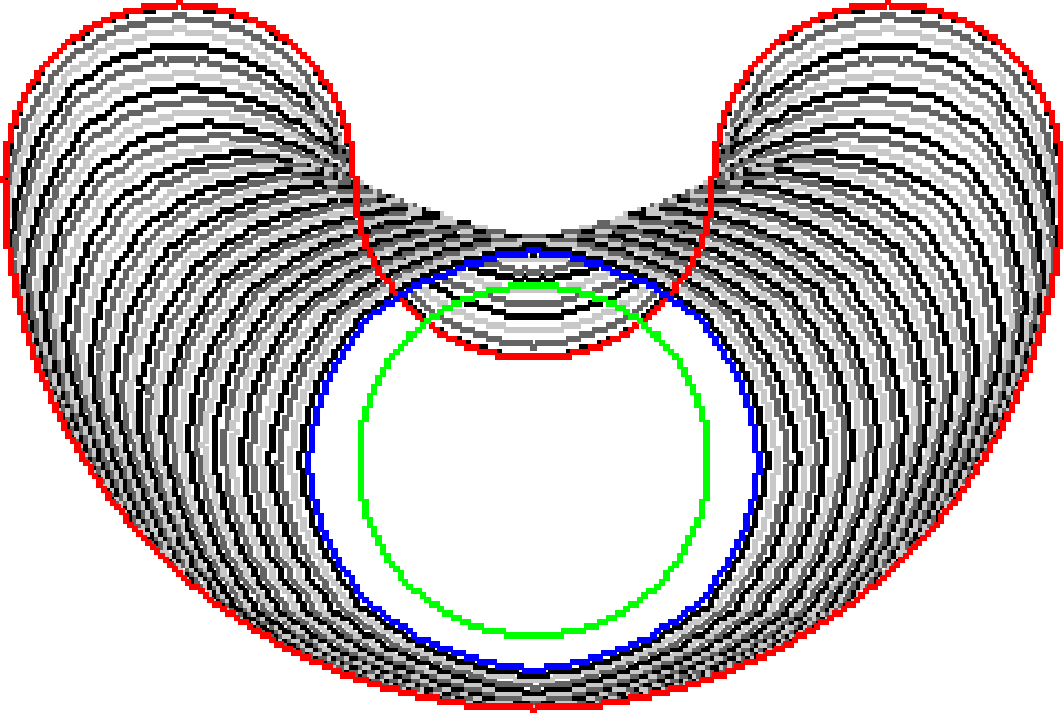
\includegraphics[scale=0.2]{figures/chapter9/free-elastica/flipflow/bean/len_pen-0.01/radius-7/summary.pdf} &
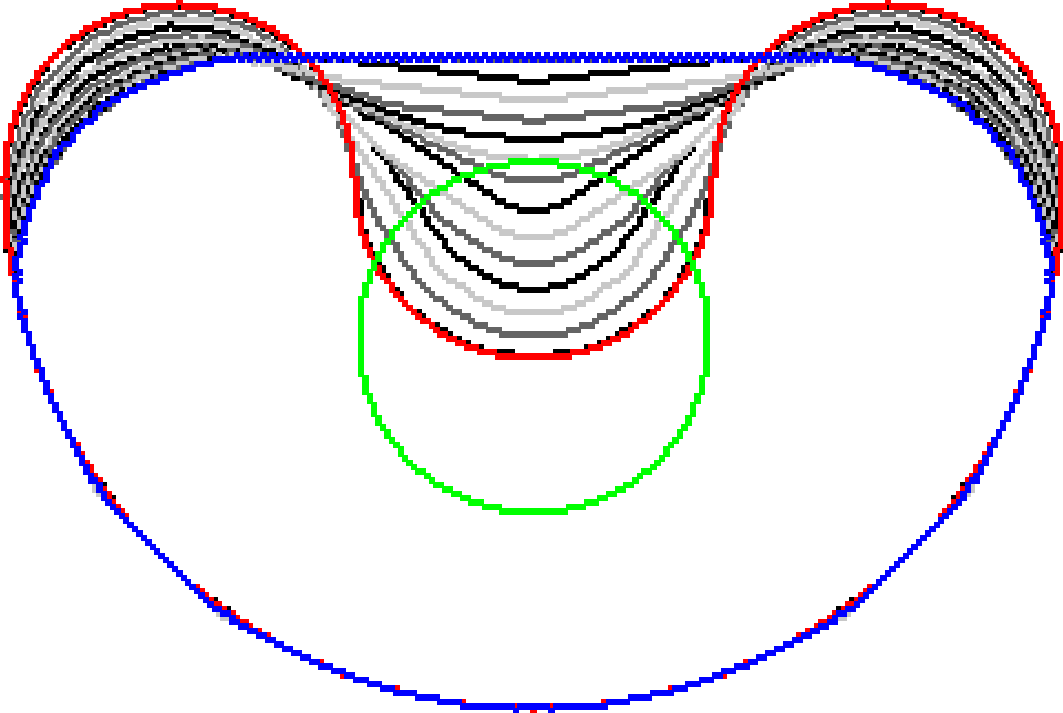
\includegraphics[scale=0.2]{figures/chapter9/free-elastica/balanceflow/bean/len_pen-0.01/radius-7/summary.pdf} &
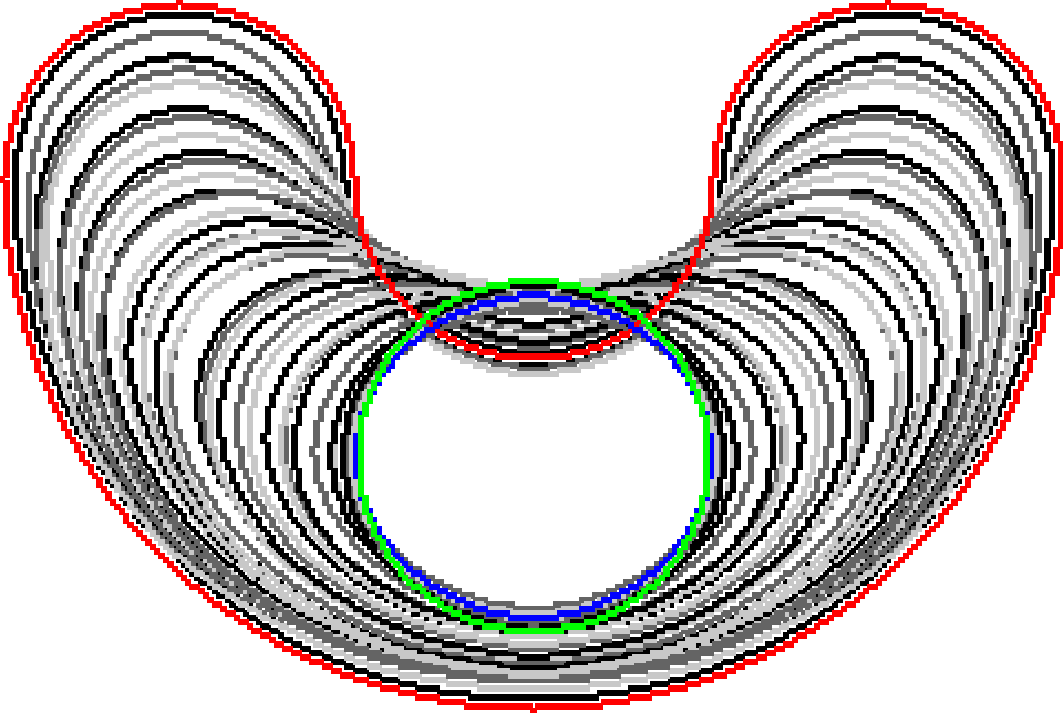
\includegraphics[scale=0.2]{figures/chapter9/free-elastica/graphflow/bean/len_pen-0.01/radius-7/summary.pdf} 
\end{tabular}
\caption{Results of Exp-General experiment for the free Elastica. Initial contour is colored in red, final contour is colored in blue and optimal contour is colored in green. Curves are drawn every $10$ iterations.}
\label{fig:results-free-elastica-general}
\end{figure}

\begin{figure}
\begin{tabular}{cc}
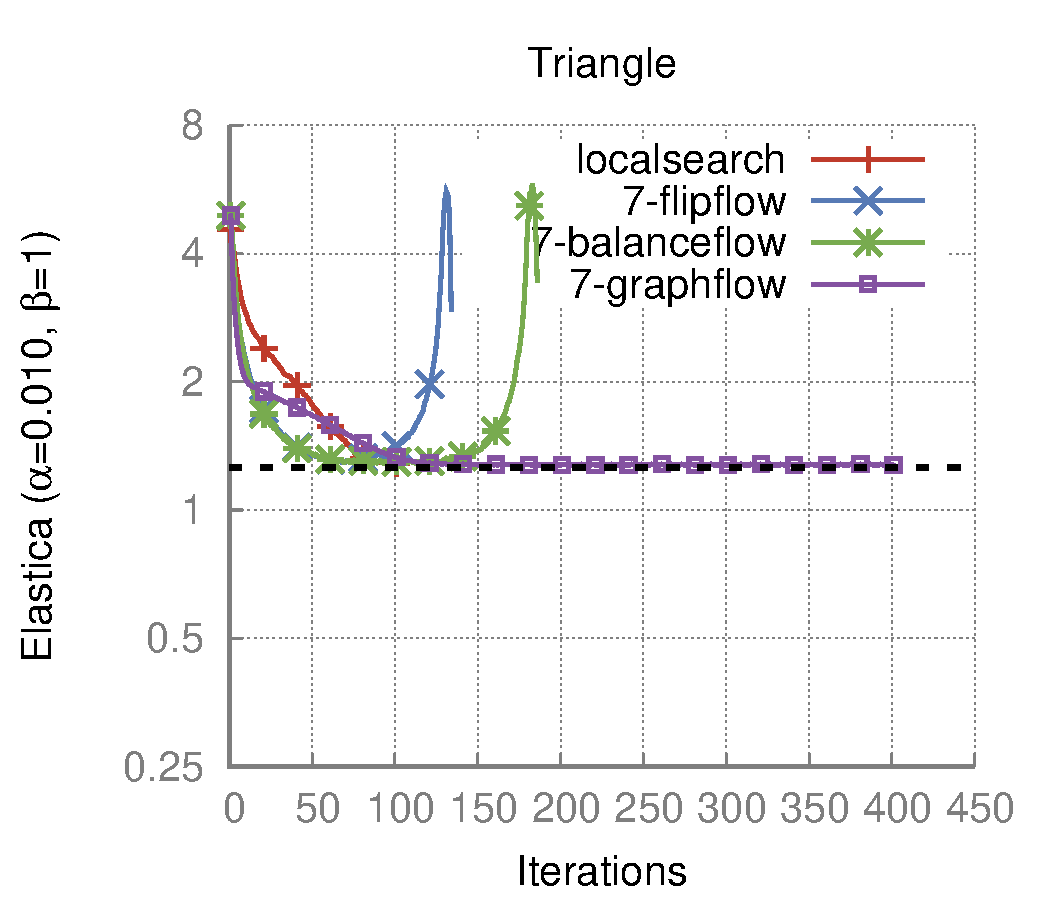
\includegraphics[scale=0.45]{figures/chapter9/free-elastica/plots/iteration/main_experiment/len_pen_0.01/radius-7/triangle.pdf} &
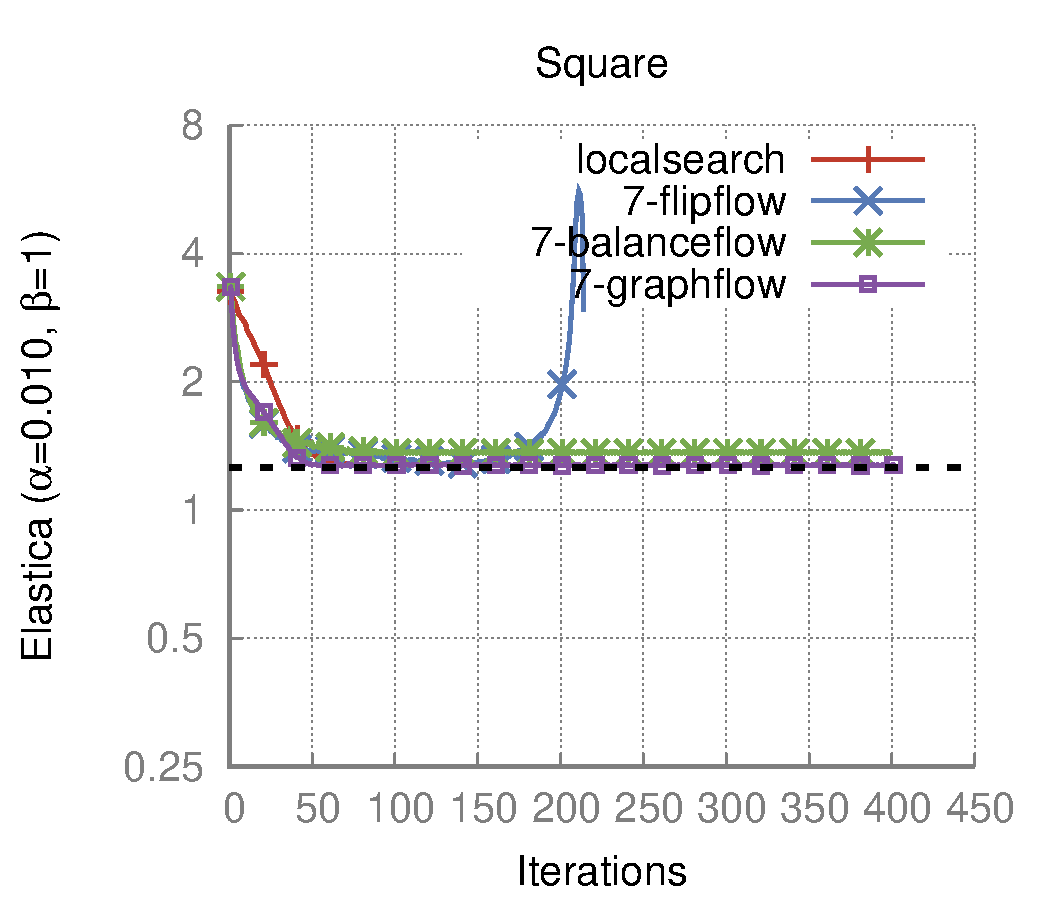
\includegraphics[scale=0.45]{figures/chapter9/free-elastica/plots/iteration/main_experiment/len_pen_0.01/radius-7/square.pdf}\\[1em]
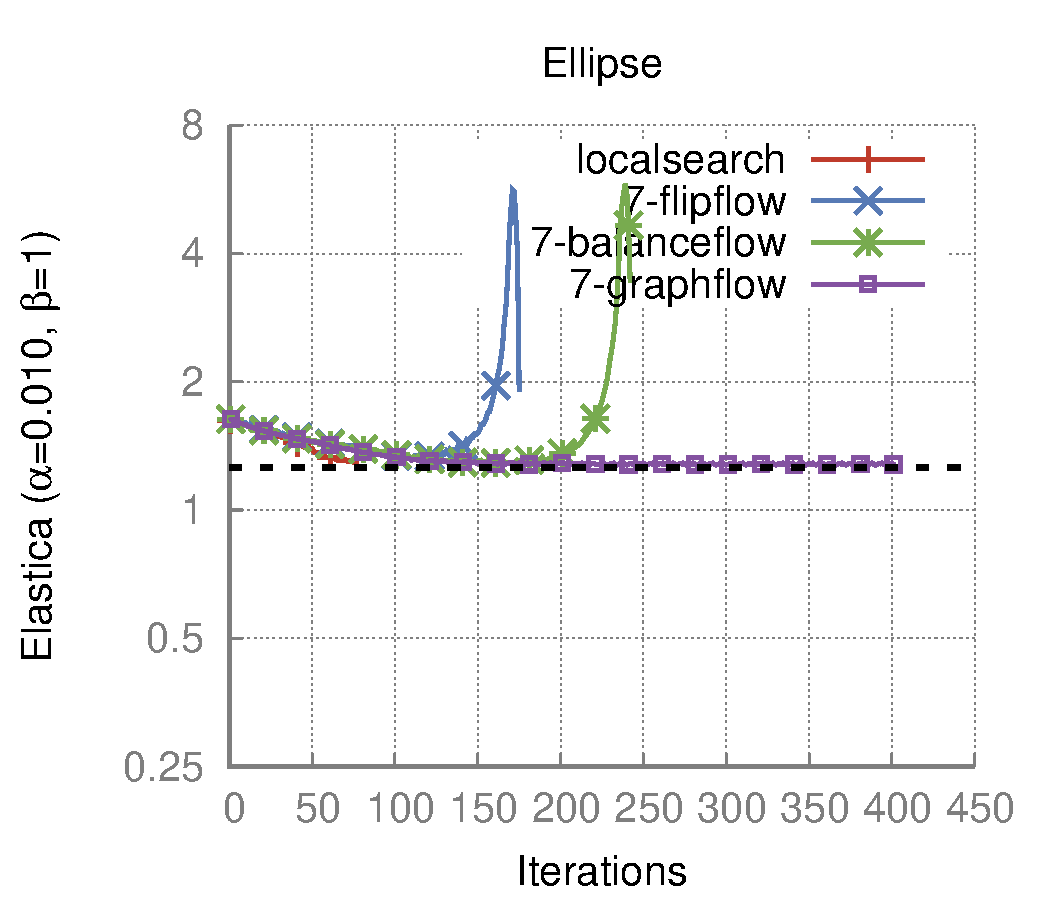
\includegraphics[scale=0.45]{figures/chapter9/free-elastica/plots/iteration/main_experiment/len_pen_0.01/radius-7/ellipse.pdf} &
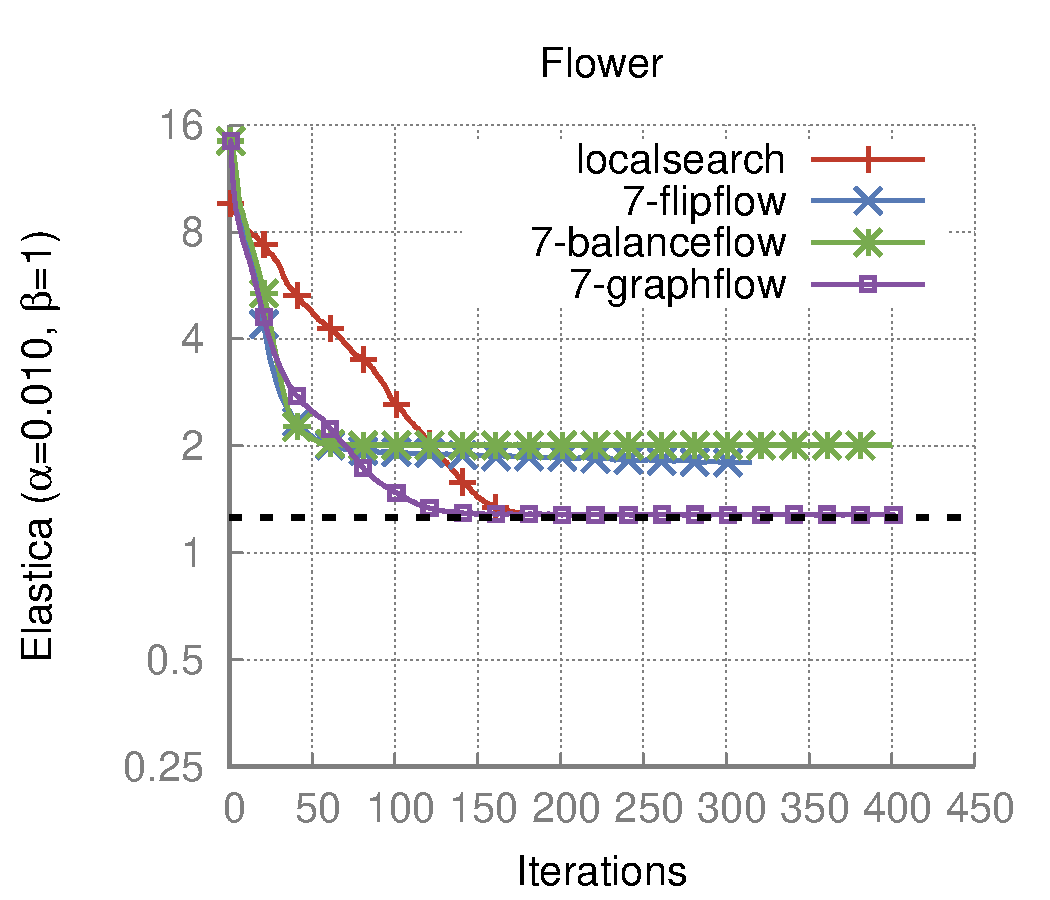
\includegraphics[scale=0.45]{figures/chapter9/free-elastica/plots/iteration/main_experiment/len_pen_0.01/radius-7/flower.pdf}\\[1em]
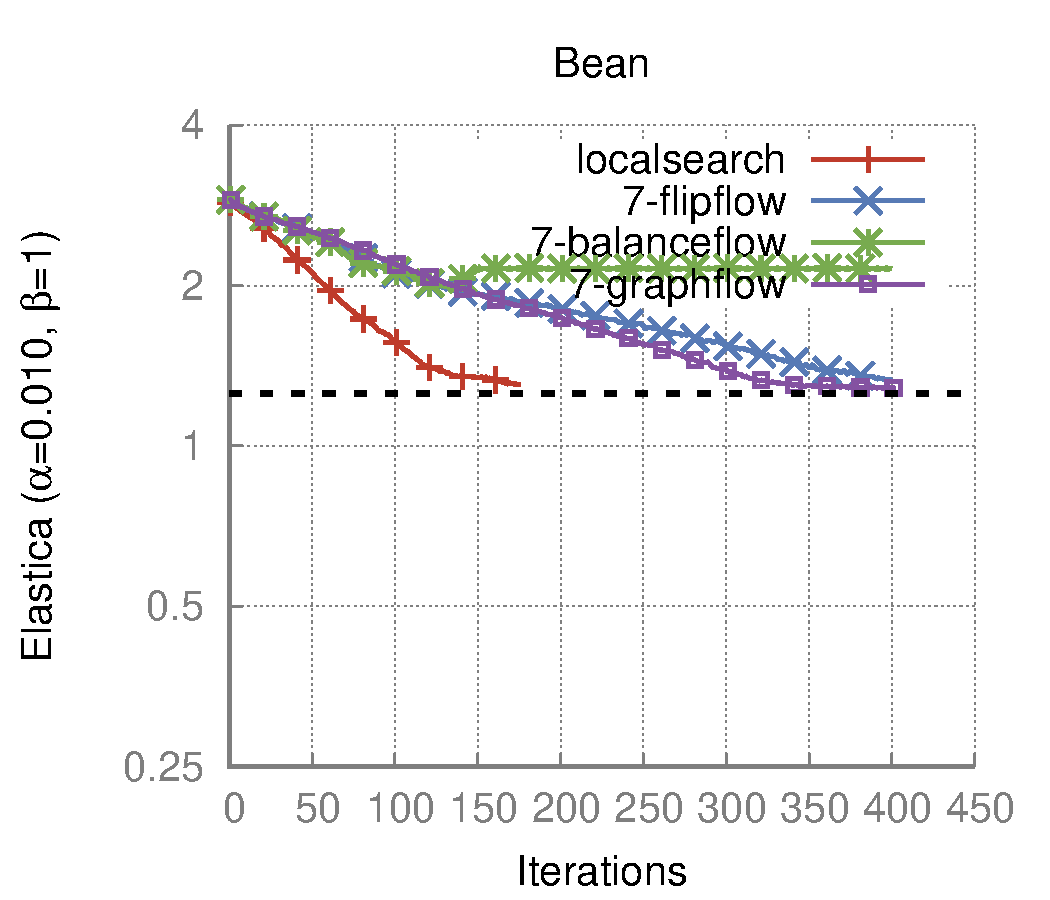
\includegraphics[scale=0.45]{figures/chapter9/free-elastica/plots/iteration/main_experiment/len_pen_0.01/radius-7/bean.pdf}
\end{tabular}
\caption{Evolution of digital Elastica value per iteration in the Exp-General experiment for the free Elastica. The dashed line marks the optimum value.}
\label{fig:plots-free-elastica-general}
\end{figure}

\subsection{Radius choice experiment}

In the Exp-Radius experiment, we set the length penalization parameter to $\alpha=0.001$. Compared to the Exp-General, the expected behaviour is that the shapes will grow till reach the optimal disk of radius $1/0.001^{0.5} \approx 31$. This experiment evidentiates the natural observation that the choice of the $bRadius$ parameter is important to the optimal shape achievement.

In the case of FlipFlow and BalanceFlow, the evolution goes faster with a larger radius, but the shape never grows, it only shrinks. On the other hand, LocalSearch and GraphFlow are sensitive to the value of $\alpha$ and they can grow or shrink the shape acoordingly. Moreover, the choice of $bRadius$ defines how closer the solution will be from the optimum.

We recall that the II estimator measures curvature by using a disk of a given radius. The radius parameter defines the range of values estimated by the estimator. At first glance, a larger radius returns a more precise estimation, but we should be careful in not use a radius larger than the shape reach at the point of estimation.

However, for the Radius-choice experiment, a value $bRadius=7$ is too small to identify the small variations that a shape that grows till become a disk of radius $31$ suffers. Therefore, when we set $bRadius=12$ both LocalSearch and GraphFlow return solutions closer to the optimal as we can check in~\cref{fig:results-free-elastica-radius-choice,fig:plots-free-elastica-radius-choice}.


\begin{figure}
\begin{tabular}{m{1.5cm}cccc}
& LocalSearch & FlipFlow & BalanceFlow & GraphFlow\\[1em]
$r=7$ & \raisebox{-.5\height}{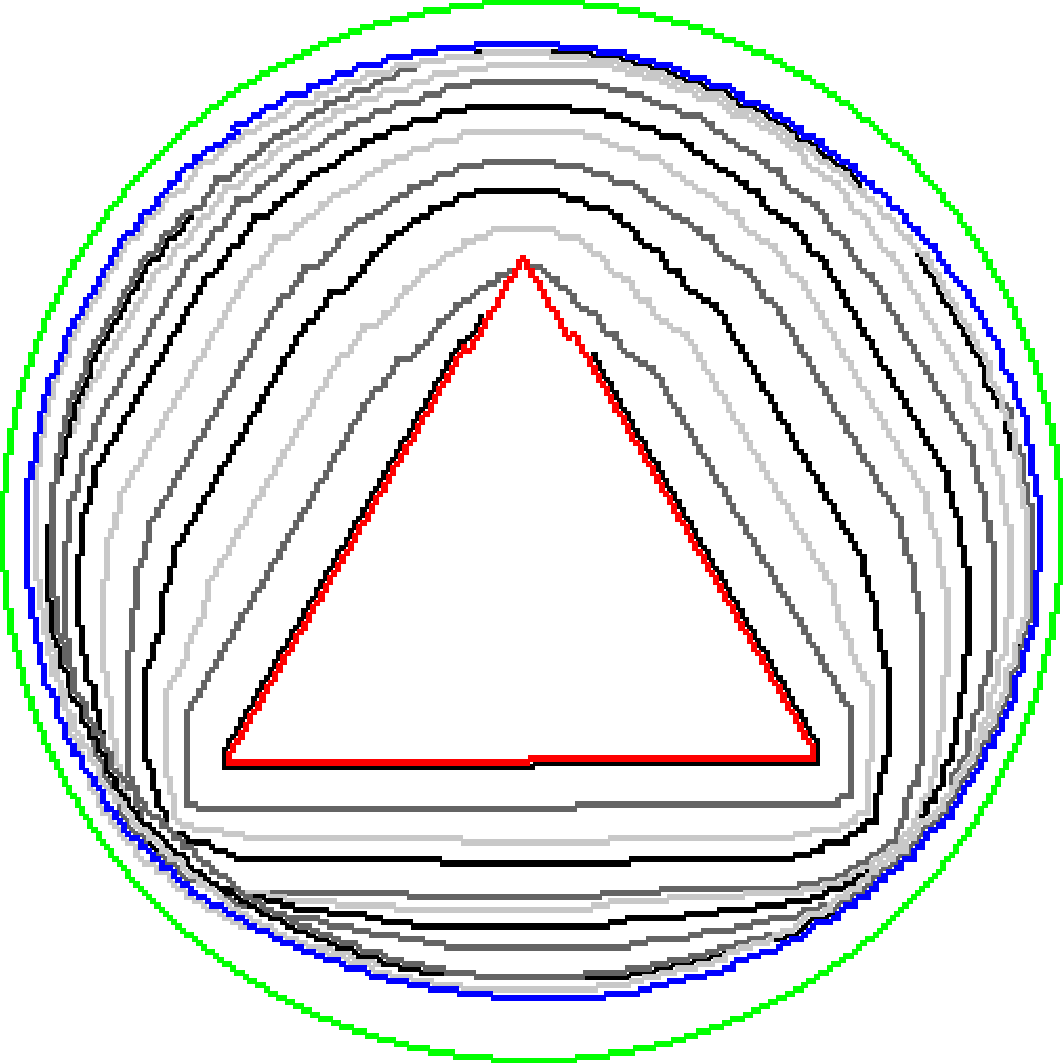
\includegraphics[scale=0.15]{figures/chapter9/free-elastica/localsearch/triangle/len_pen-0.001/radius-7/summary.pdf}} & 
\raisebox{-.5\height}{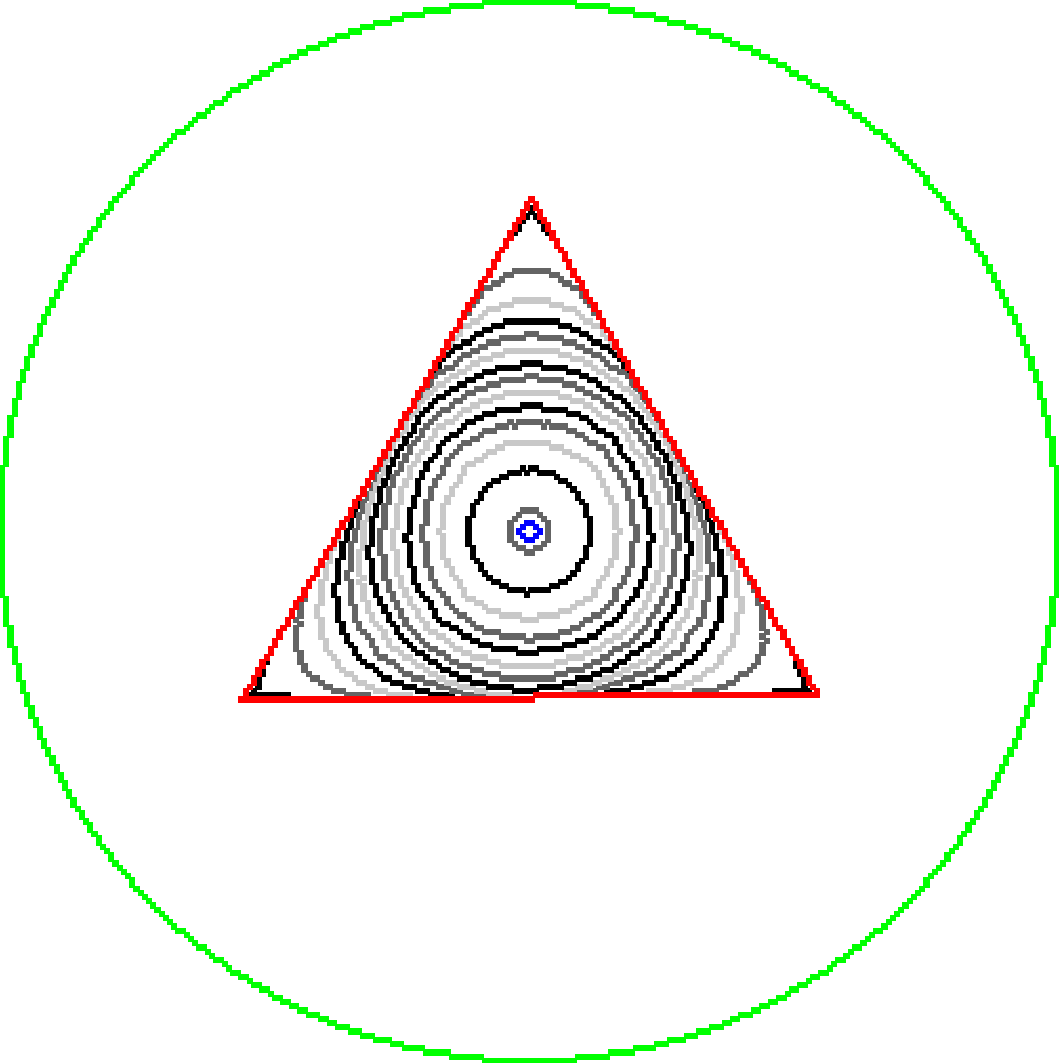
\includegraphics[scale=0.15]{figures/chapter9/free-elastica/flipflow/triangle/len_pen-0.001/radius-7/summary.pdf}} &
\raisebox{-.5\height}{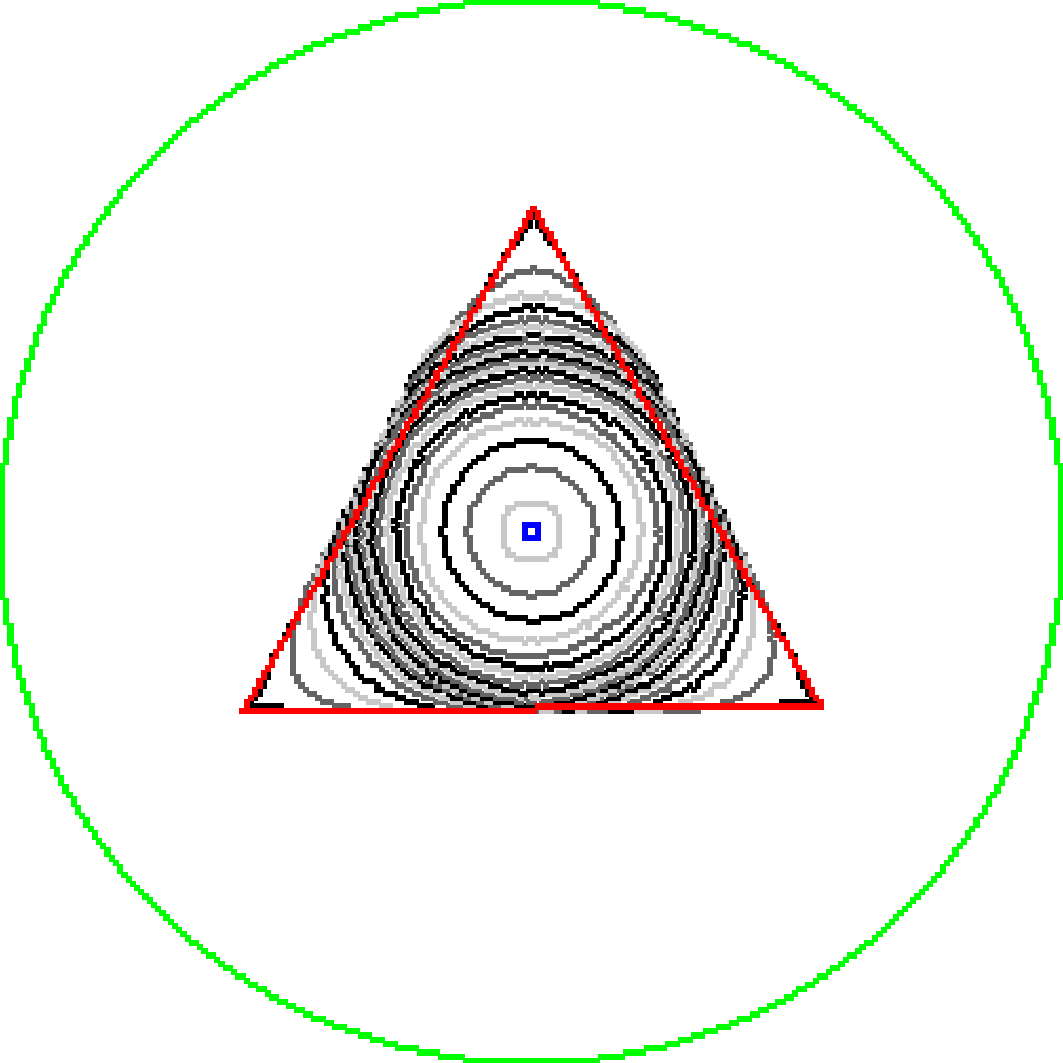
\includegraphics[scale=0.15]{figures/chapter9/free-elastica/balanceflow/triangle/len_pen-0.001/radius-7/summary.pdf}} &
\raisebox{-.5\height}{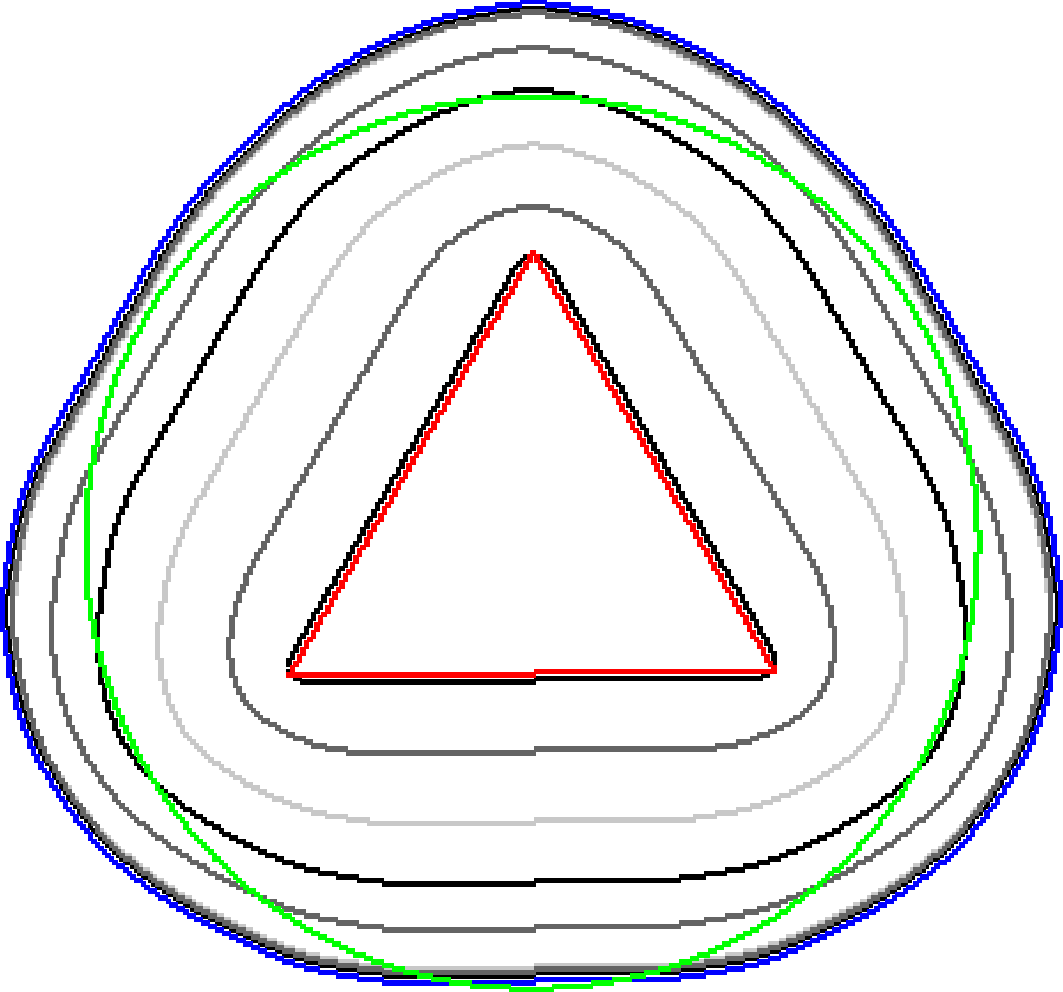
\includegraphics[scale=0.15]{figures/chapter9/free-elastica/graphflow/triangle/len_pen-0.001/radius-7/summary.pdf}} \\[4em]
$r=12$ & \raisebox{-.5\height}{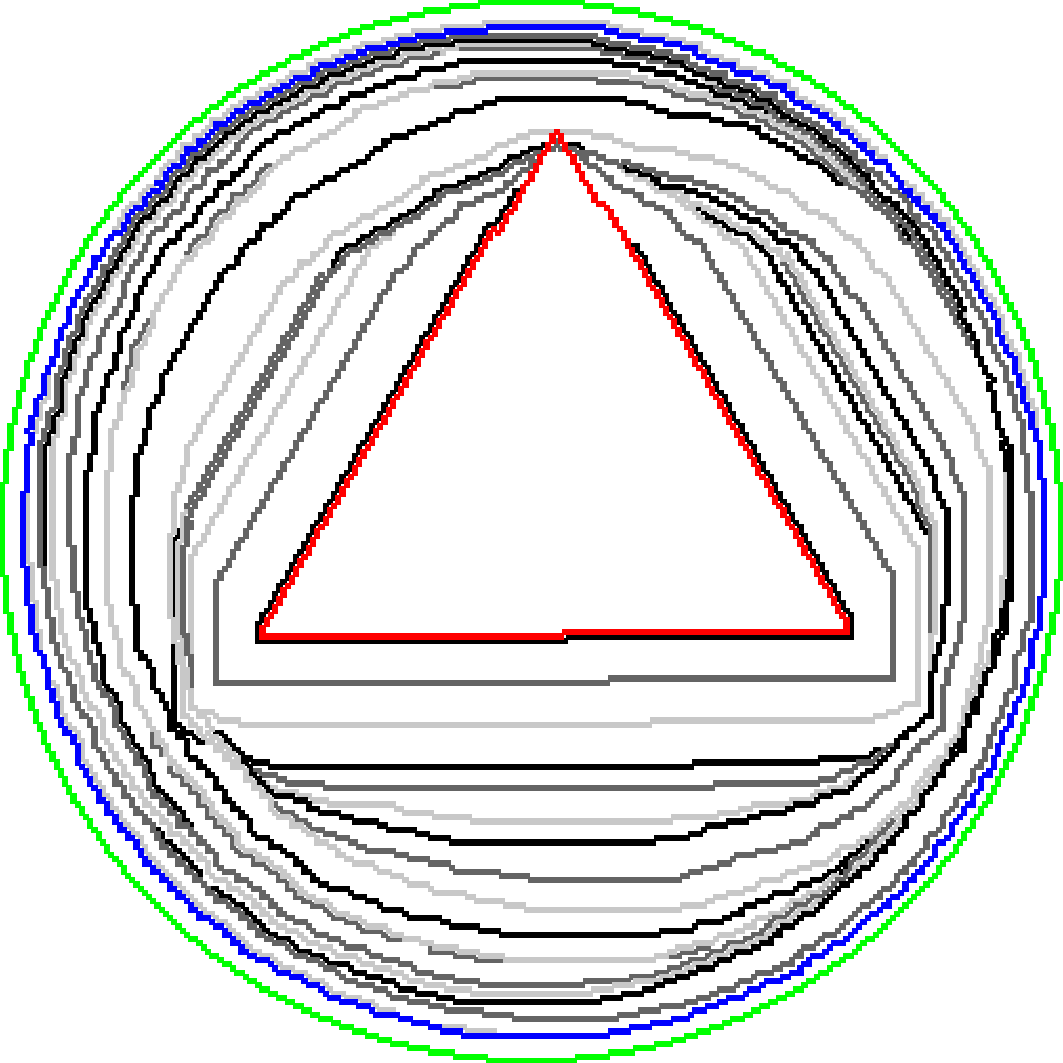
\includegraphics[scale=0.15]{figures/chapter9/free-elastica/localsearch/triangle/len_pen-0.001/radius-12/summary.pdf}} & 
\raisebox{-.5\height}{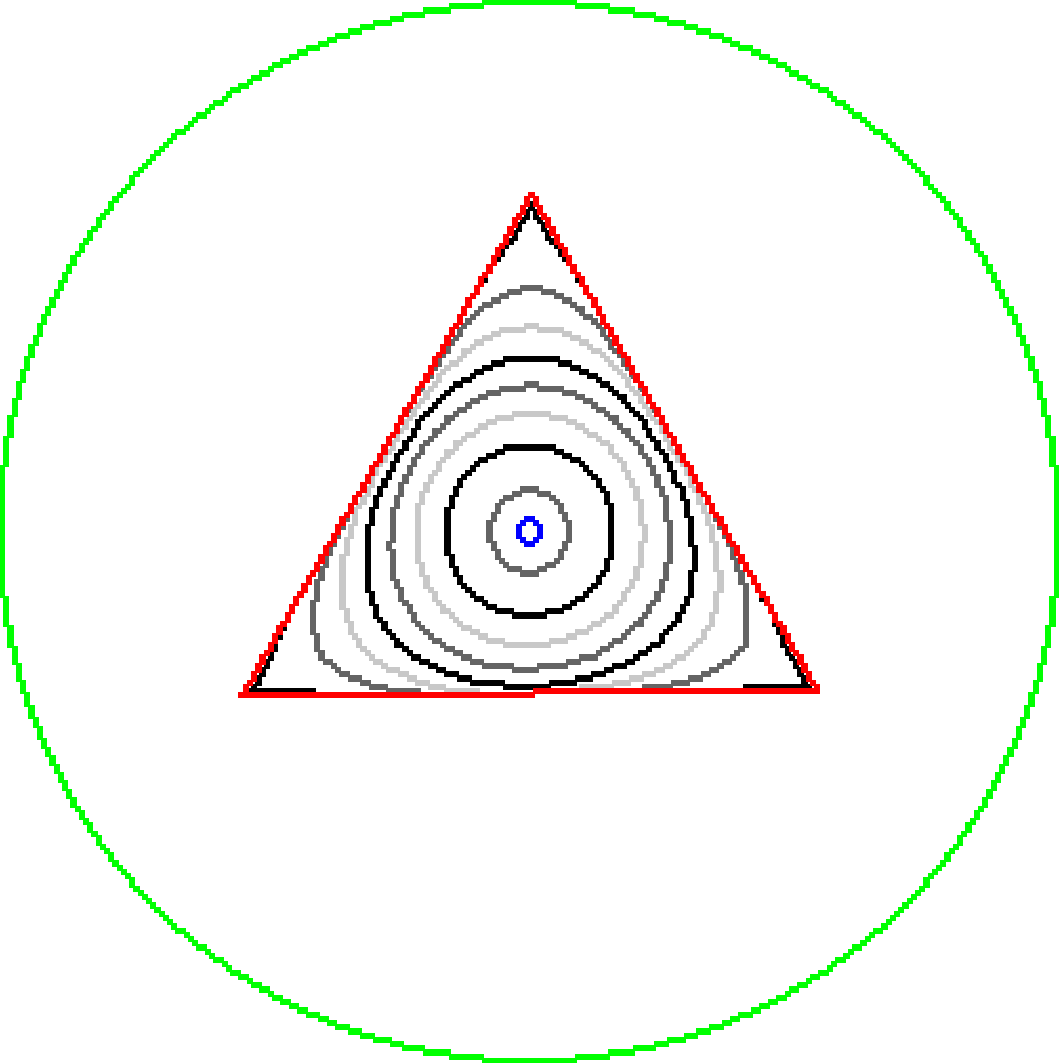
\includegraphics[scale=0.15]{figures/chapter9/free-elastica/flipflow/triangle/len_pen-0.001/radius-12/summary.pdf}} &
\raisebox{-.5\height}{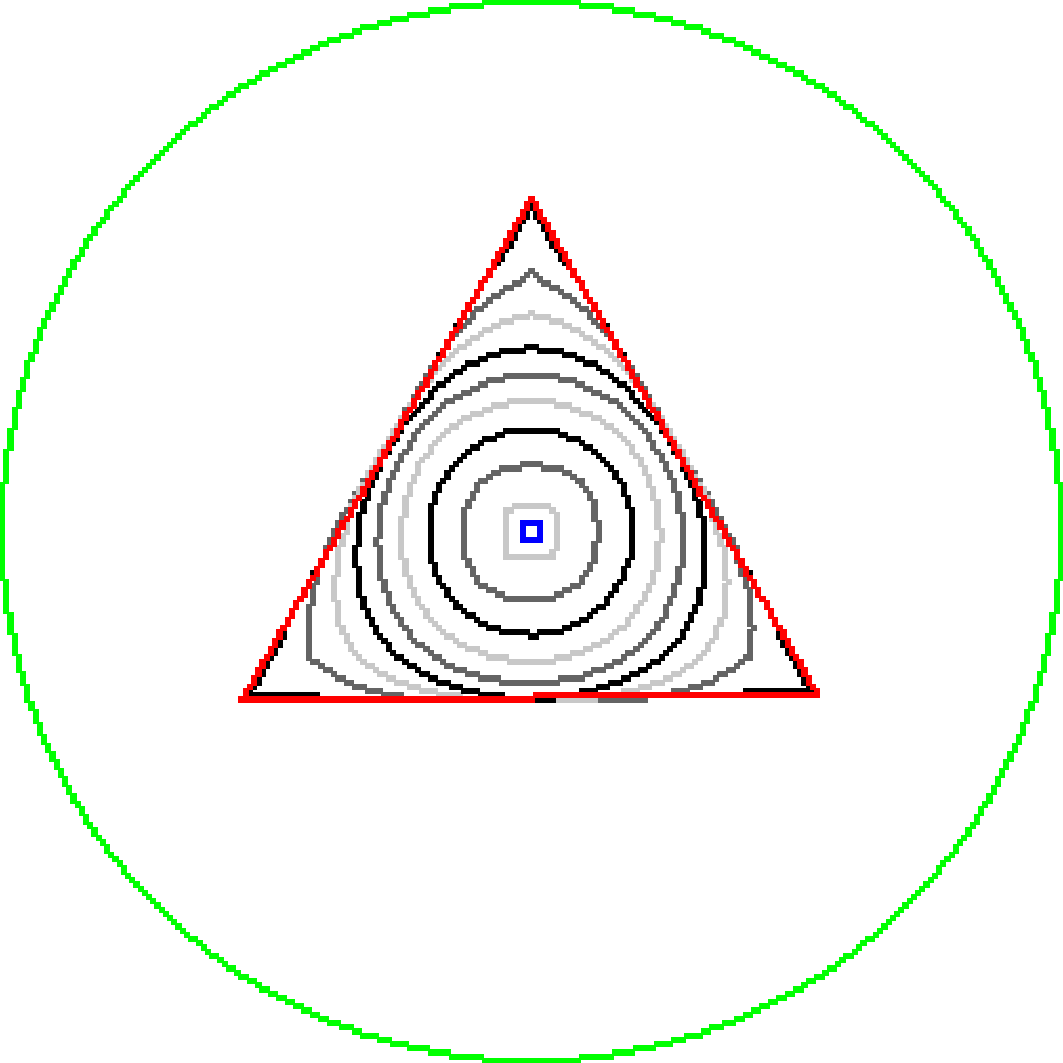
\includegraphics[scale=0.15]{figures/chapter9/free-elastica/balanceflow/triangle/len_pen-0.001/radius-12/summary.pdf}} &
\raisebox{-.5\height}{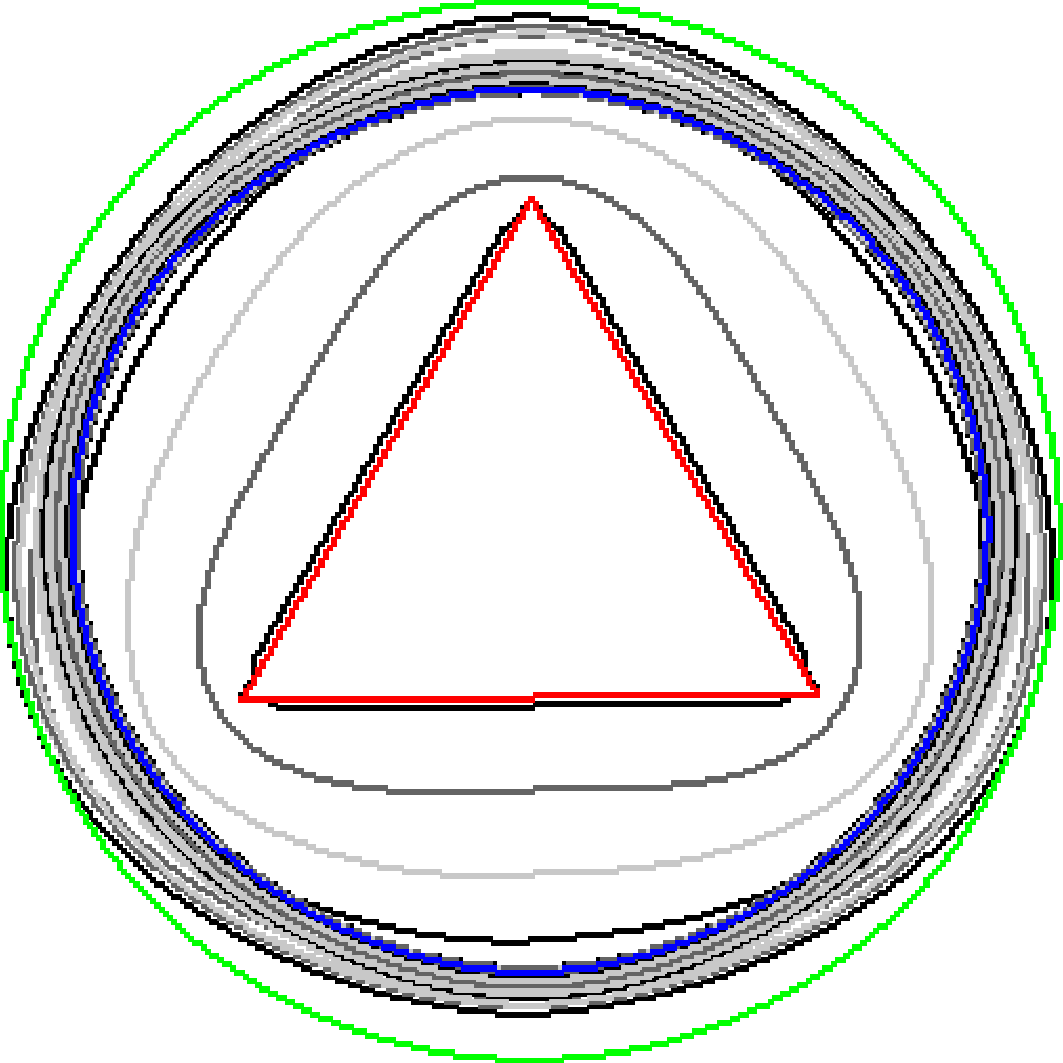
\includegraphics[scale=0.15]{figures/chapter9/free-elastica/graphflow/triangle/len_pen-0.001/radius-12/summary.pdf}} \\[4em]
$r=7$ & \raisebox{-.5\height}{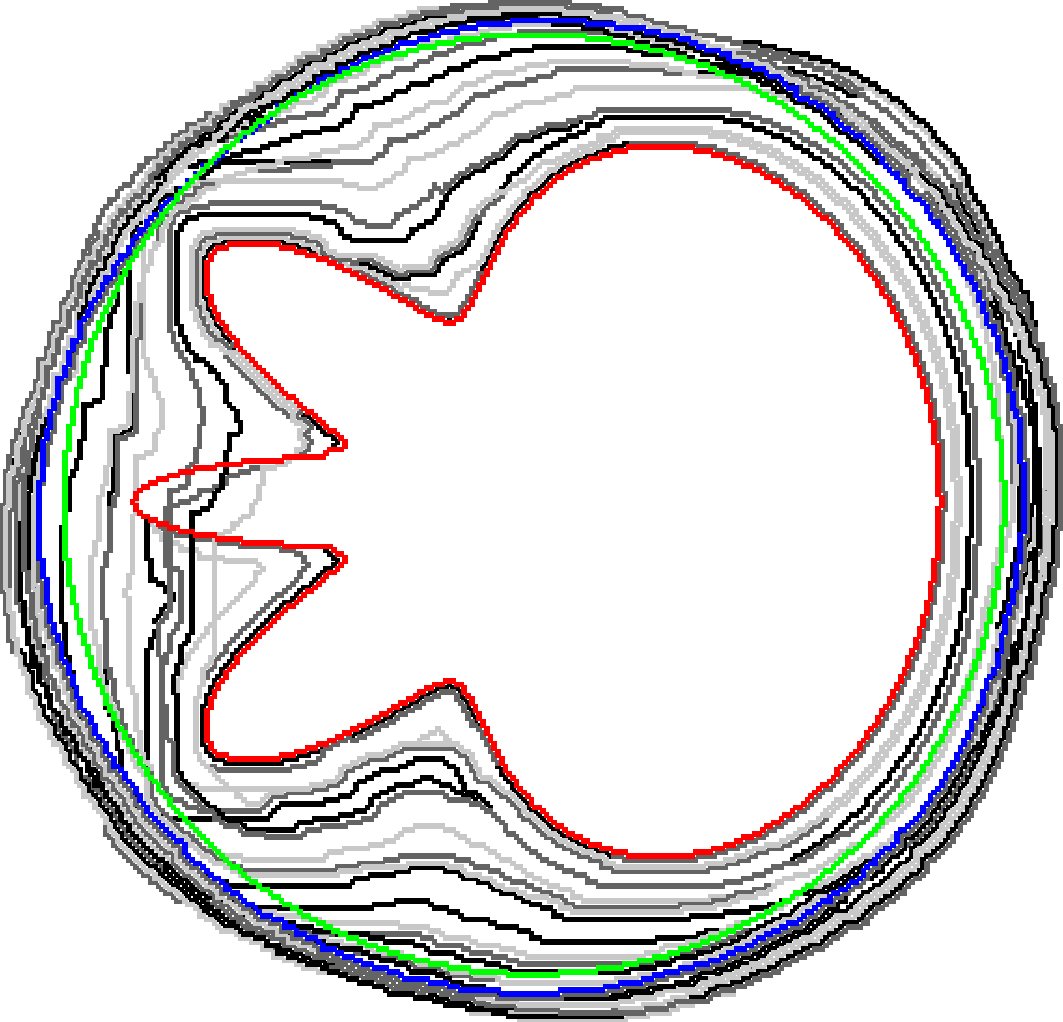
\includegraphics[scale=0.15]{figures/chapter9/free-elastica/localsearch/flower/len_pen-0.001/radius-7/summary.pdf}} & 
\raisebox{-.5\height}{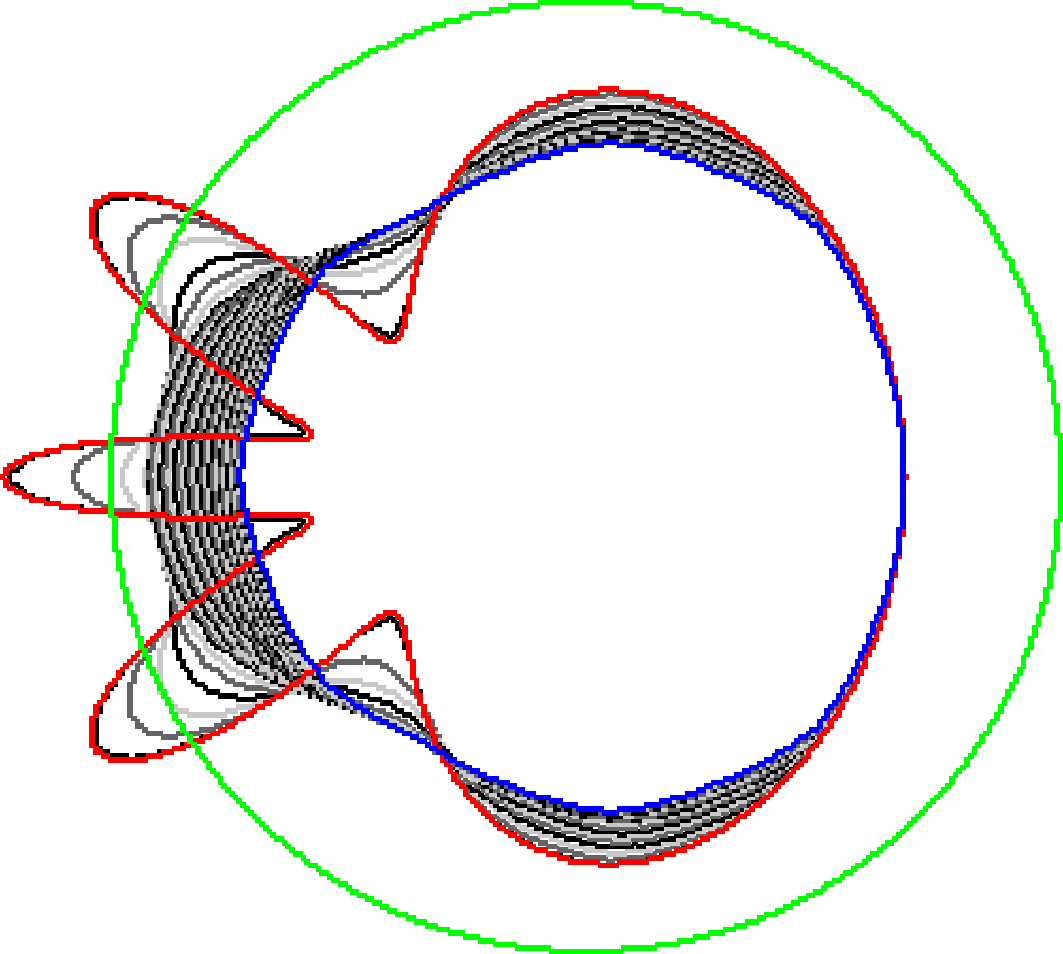
\includegraphics[scale=0.15]{figures/chapter9/free-elastica/flipflow/flower/len_pen-0.001/radius-7/summary.pdf}} &
\raisebox{-.5\height}{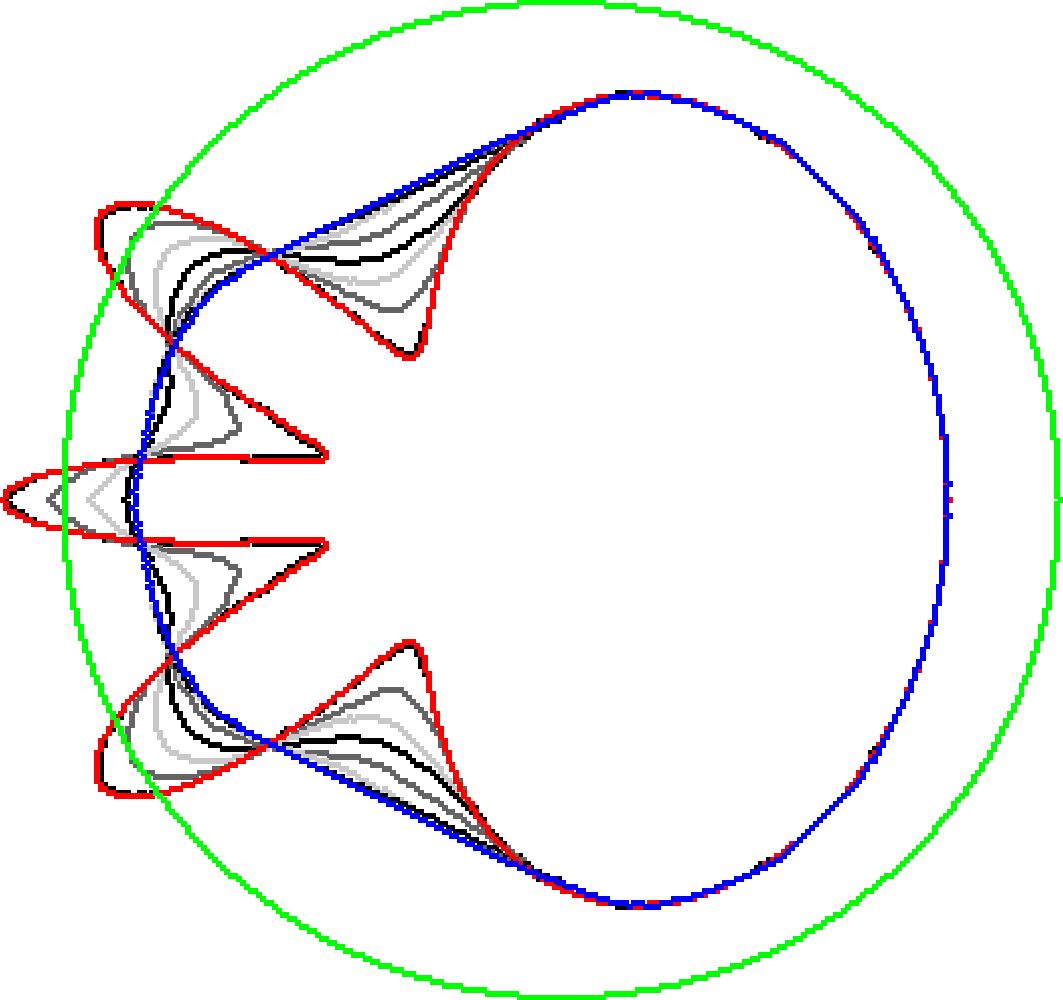
\includegraphics[scale=0.15]{figures/chapter9/free-elastica/balanceflow/flower/len_pen-0.001/radius-7/summary.pdf}} &
\raisebox{-.5\height}{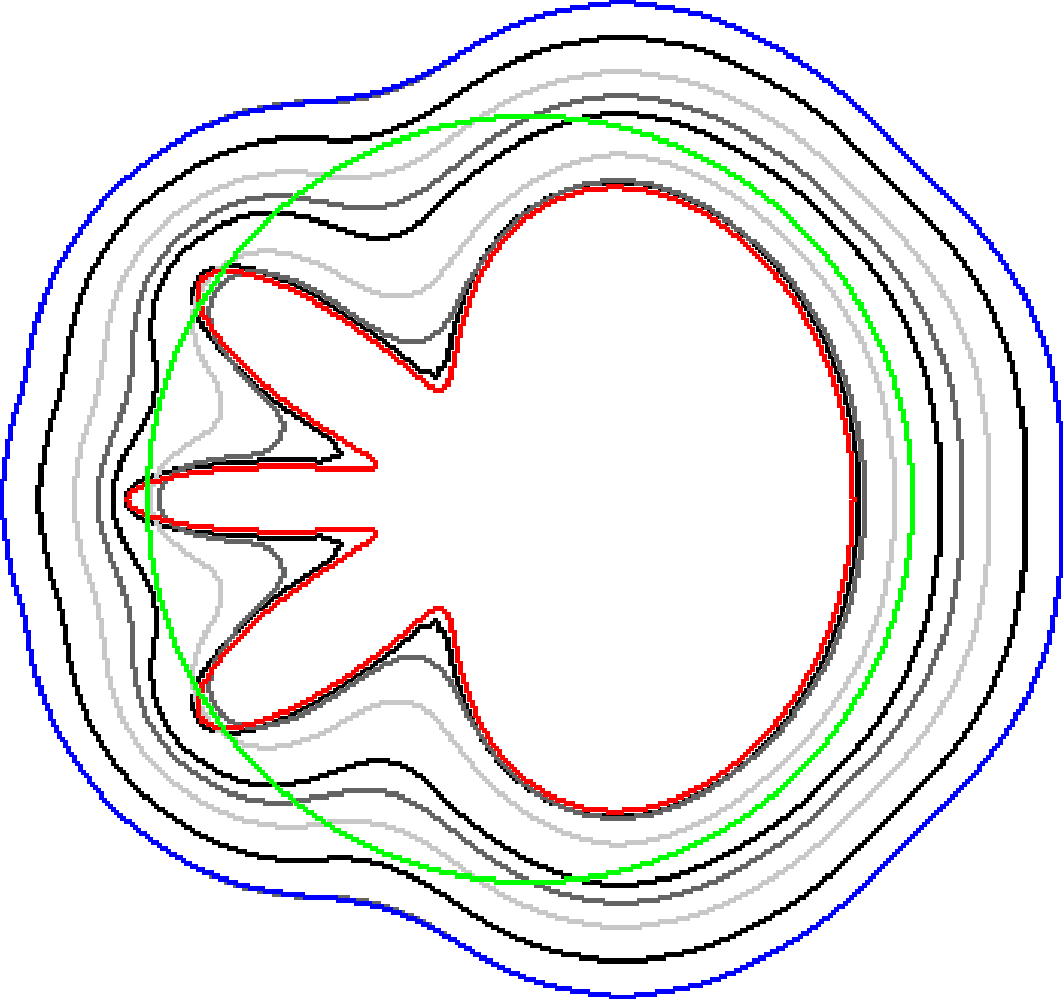
\includegraphics[scale=0.15]{figures/chapter9/free-elastica/graphflow/flower/len_pen-0.001/radius-7/summary.pdf}} \\[4em]
$r=12$ & \raisebox{-.5\height}{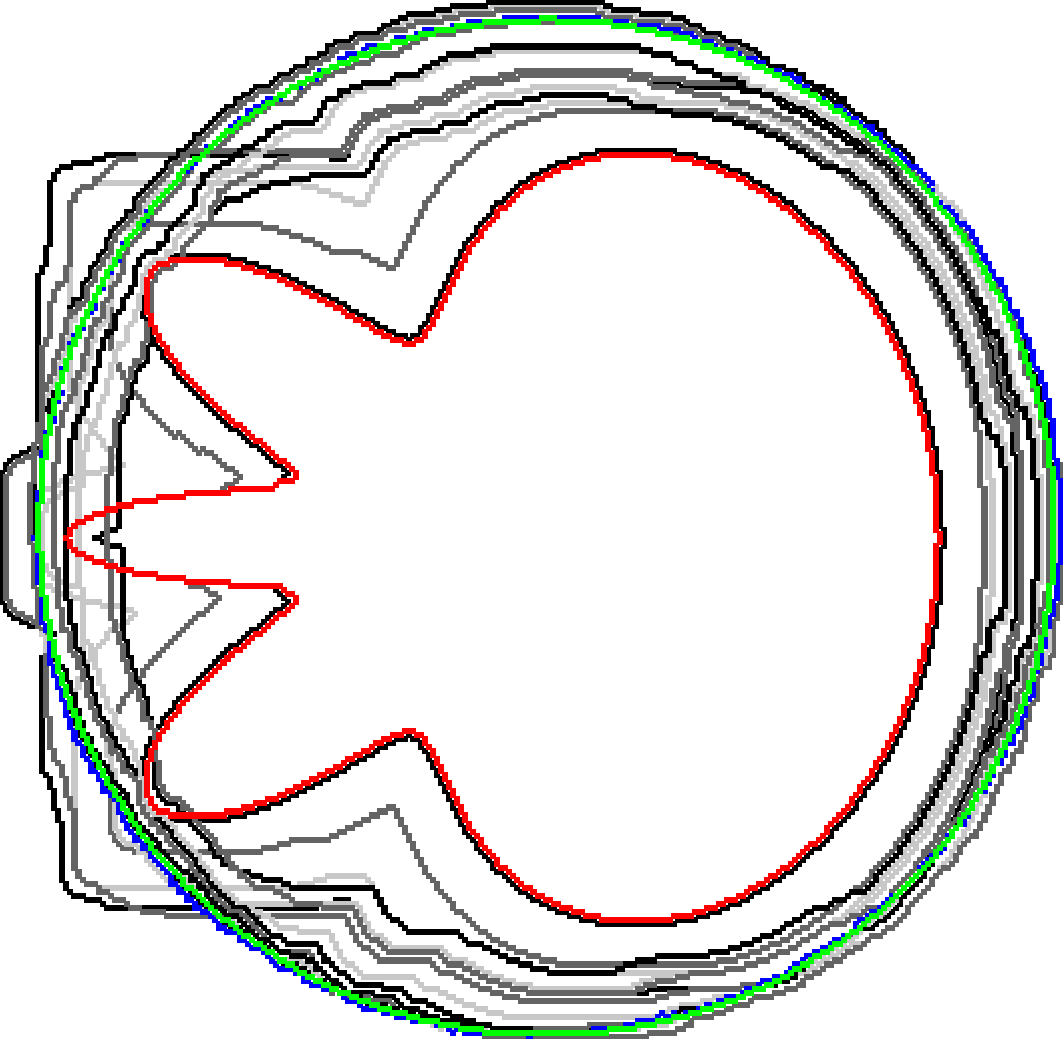
\includegraphics[scale=0.15]{figures/chapter9/free-elastica/localsearch/flower/len_pen-0.001/radius-12/summary.pdf}} & 
\raisebox{-.5\height}{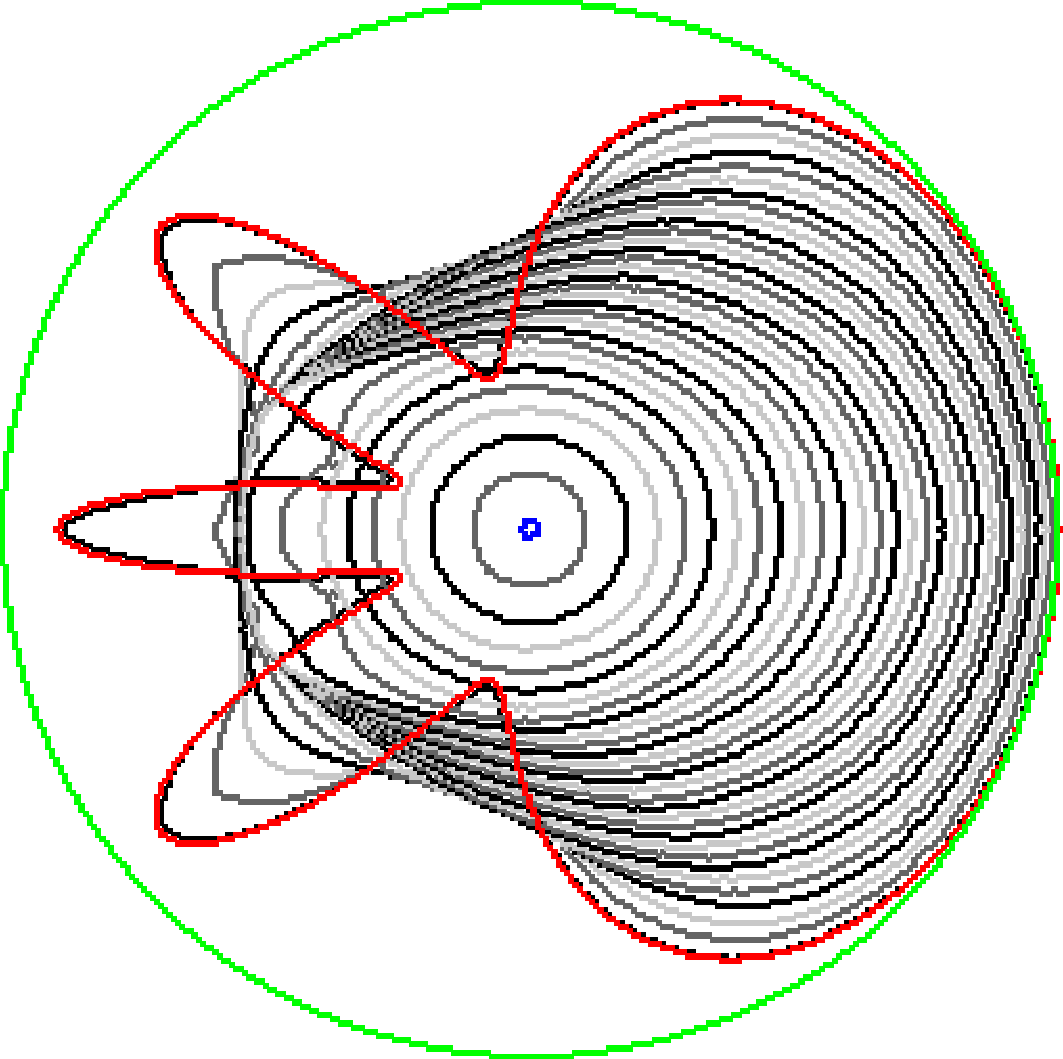
\includegraphics[scale=0.15]{figures/chapter9/free-elastica/flipflow/flower/len_pen-0.001/radius-12/summary.pdf}} &
\raisebox{-.5\height}{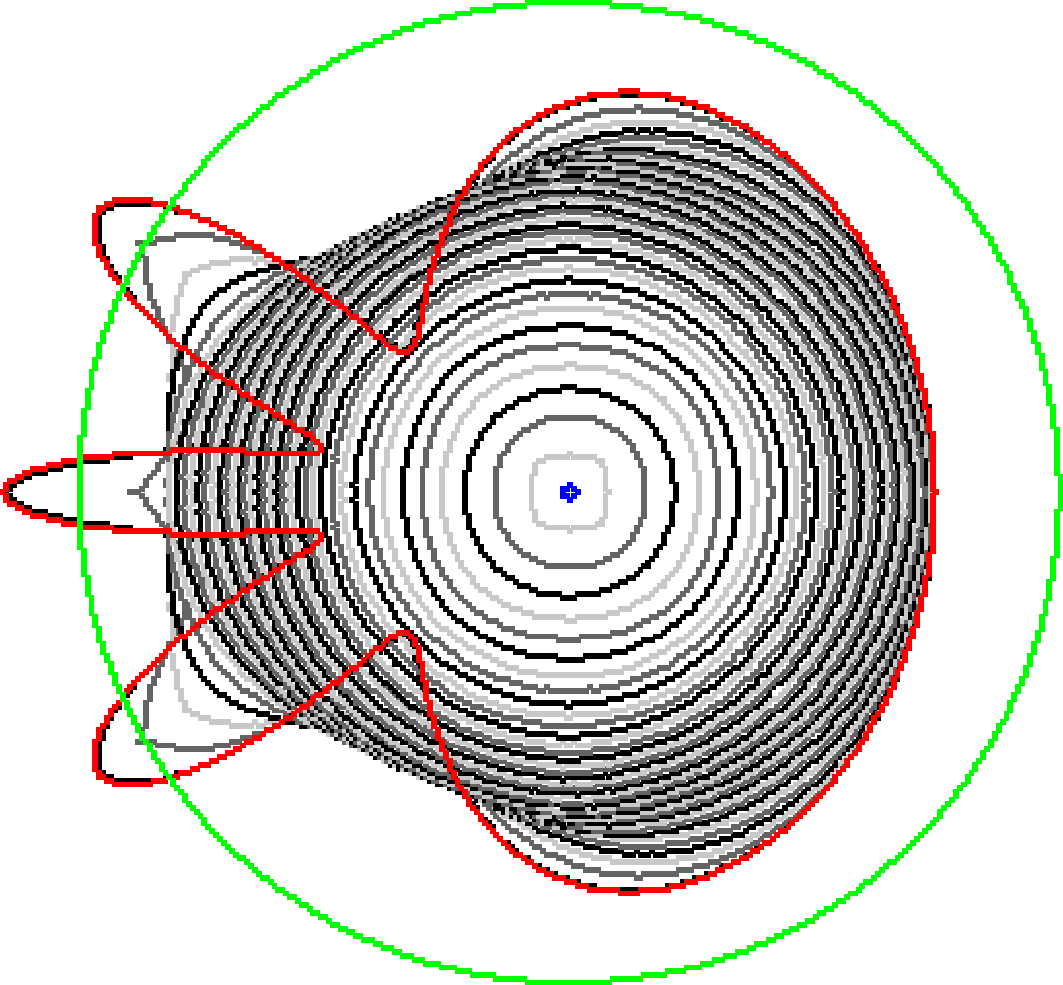
\includegraphics[scale=0.15]{figures/chapter9/free-elastica/balanceflow/flower/len_pen-0.001/radius-12/summary.pdf}} &
\raisebox{-.5\height}{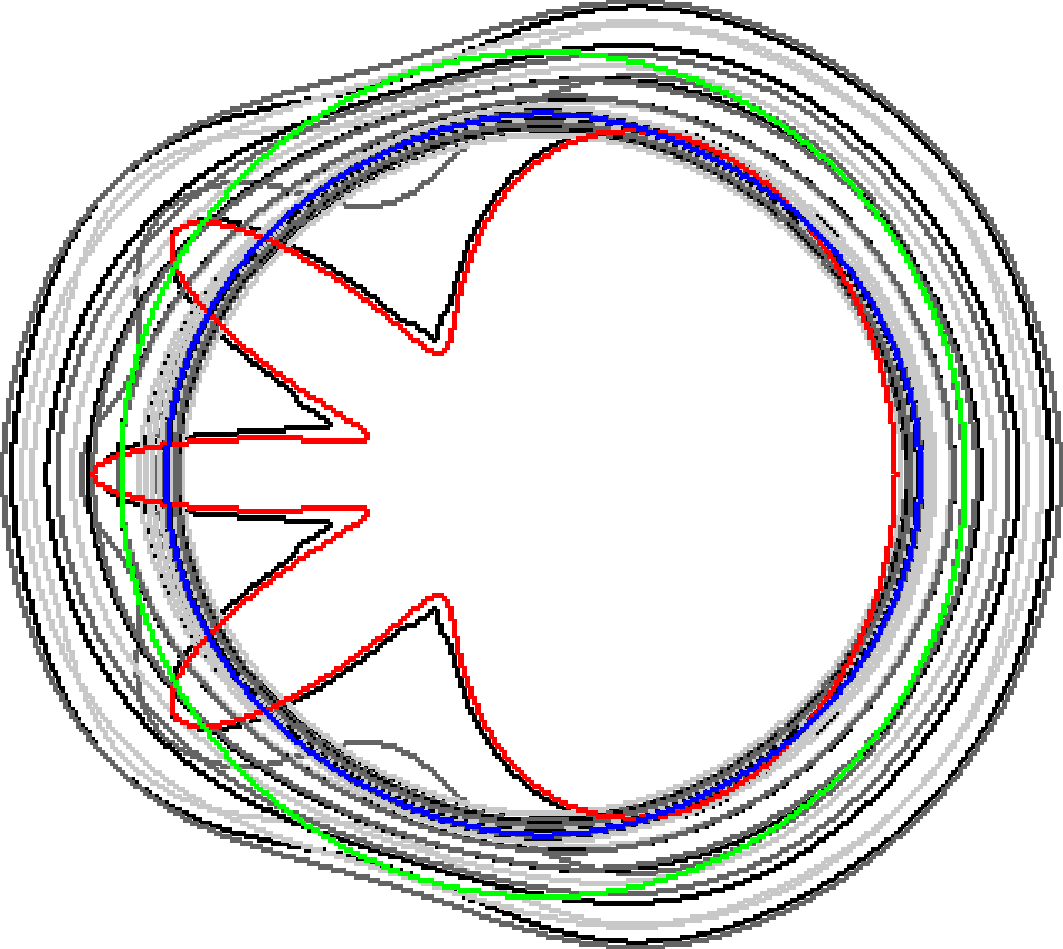
\includegraphics[scale=0.15]{figures/chapter9/free-elastica/graphflow/flower/len_pen-0.001/radius-12/summary.pdf}}
\end{tabular}
\caption{Results of Exp-Radius experiment for the free Elastica. Initial contour is colored in red, final contour is colored in blue and optimal contour is colored in green. Curves are drawn every $10$ iterations.}
\label{fig:results-free-elastica-radius-choice}
\end{figure}

\begin{figure}
\begin{tabular}{cc}
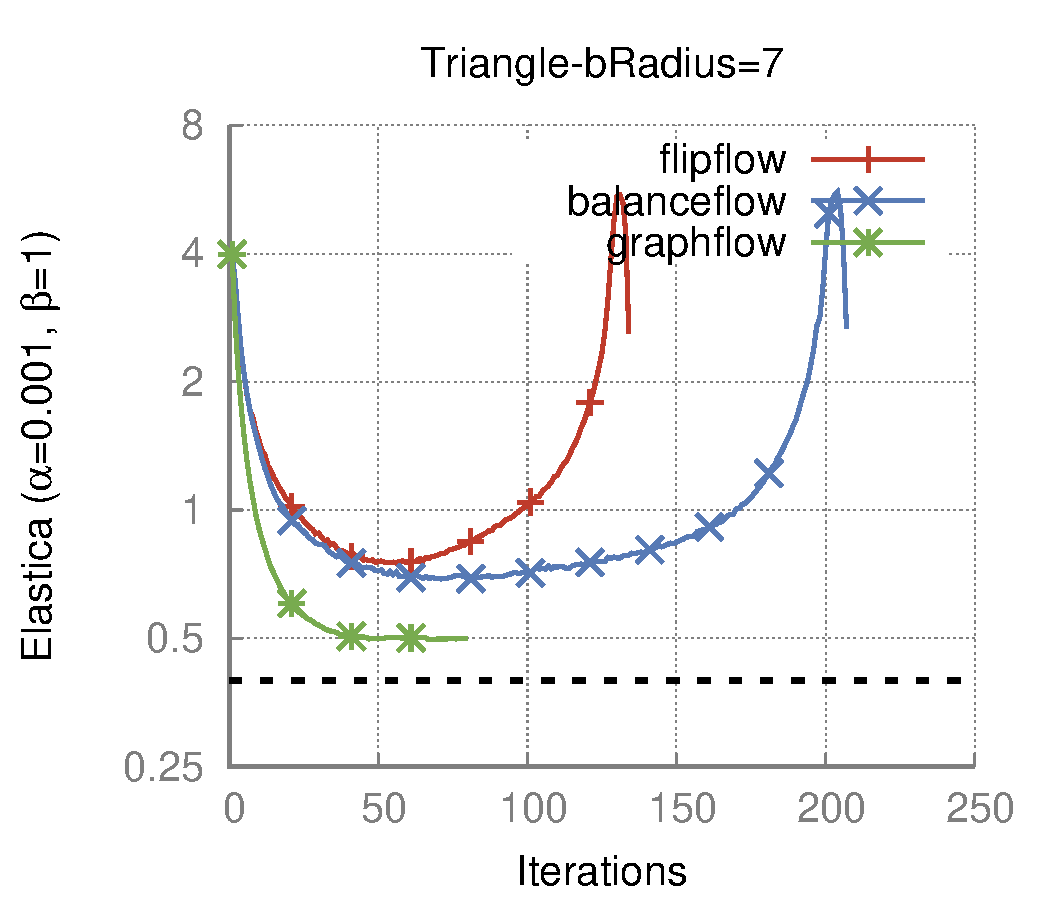
\includegraphics[scale=0.4]{figures/chapter9/free-elastica/plots/iteration/radius_choice/len_pen_0.001/radius-7/triangle.pdf} & 
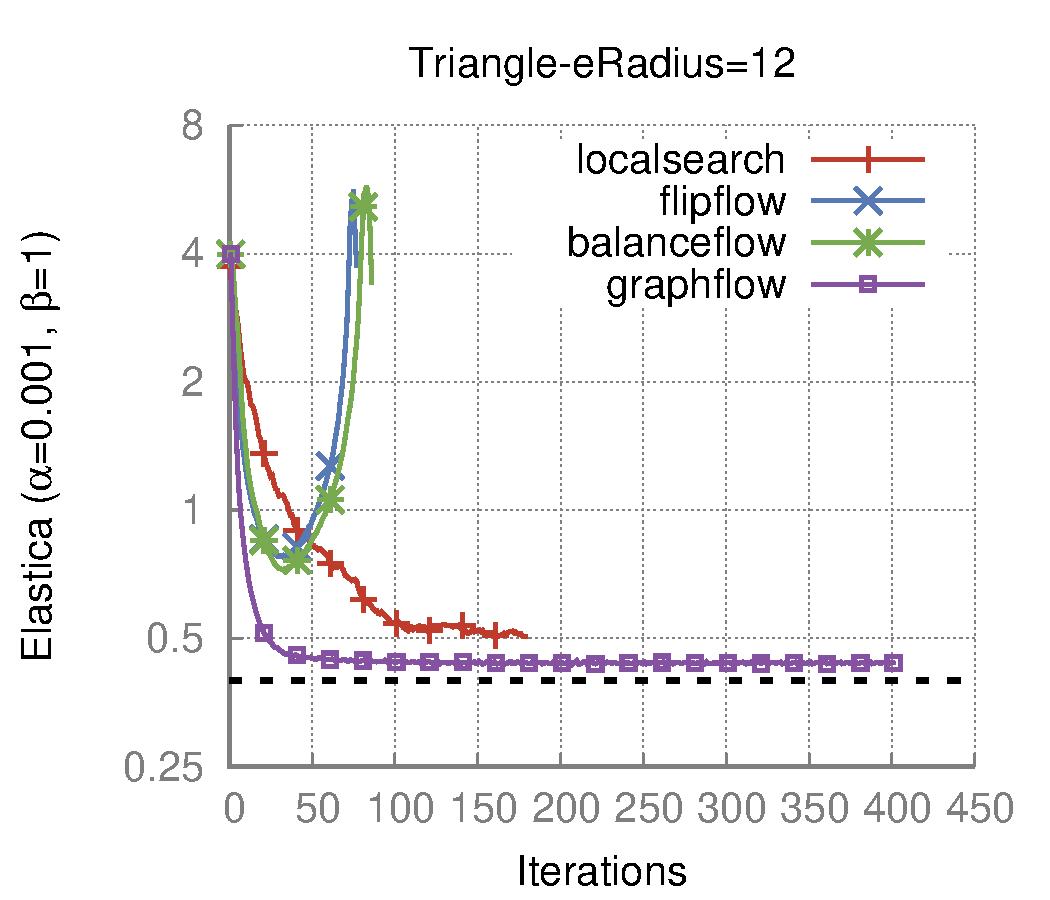
\includegraphics[scale=0.4]{figures/chapter9/free-elastica/plots/iteration/radius_choice/len_pen_0.001/radius-12/triangle.pdf}\\[1em] 
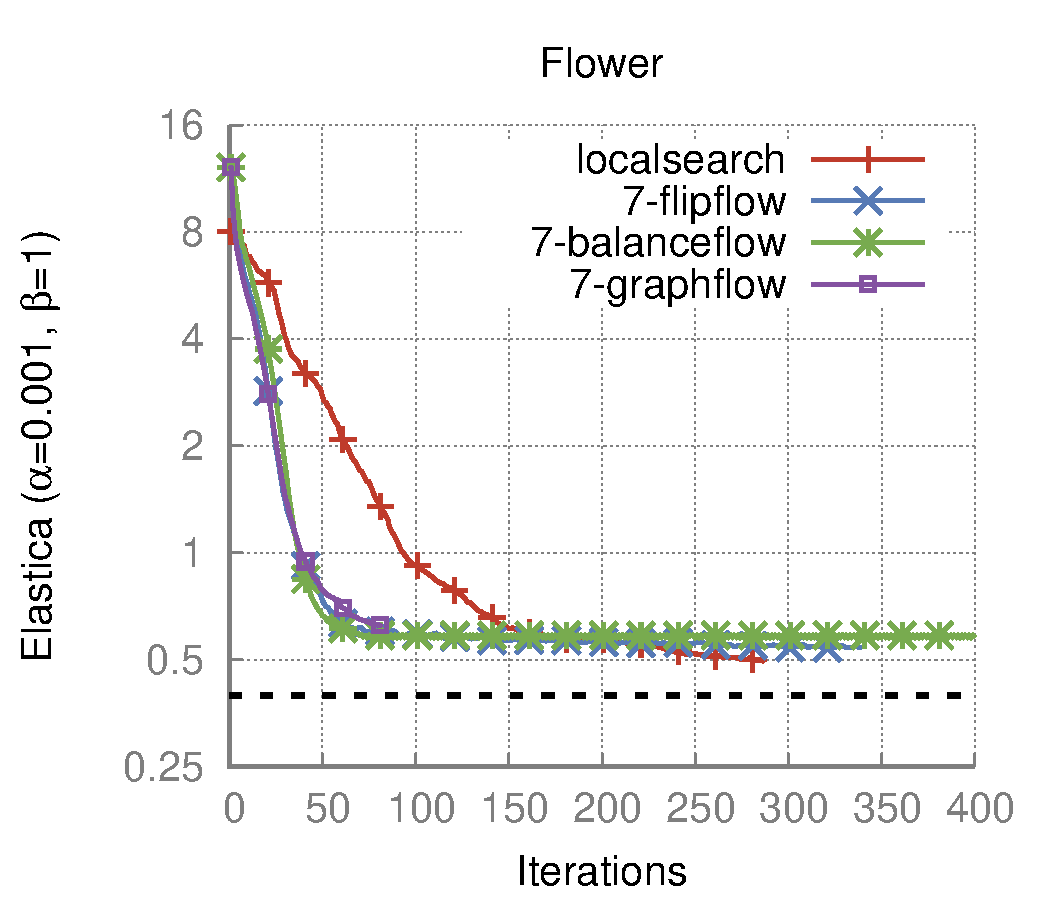
\includegraphics[scale=0.4]{figures/chapter9/free-elastica/plots/iteration/radius_choice/len_pen_0.001/radius-7/flower.pdf} & 
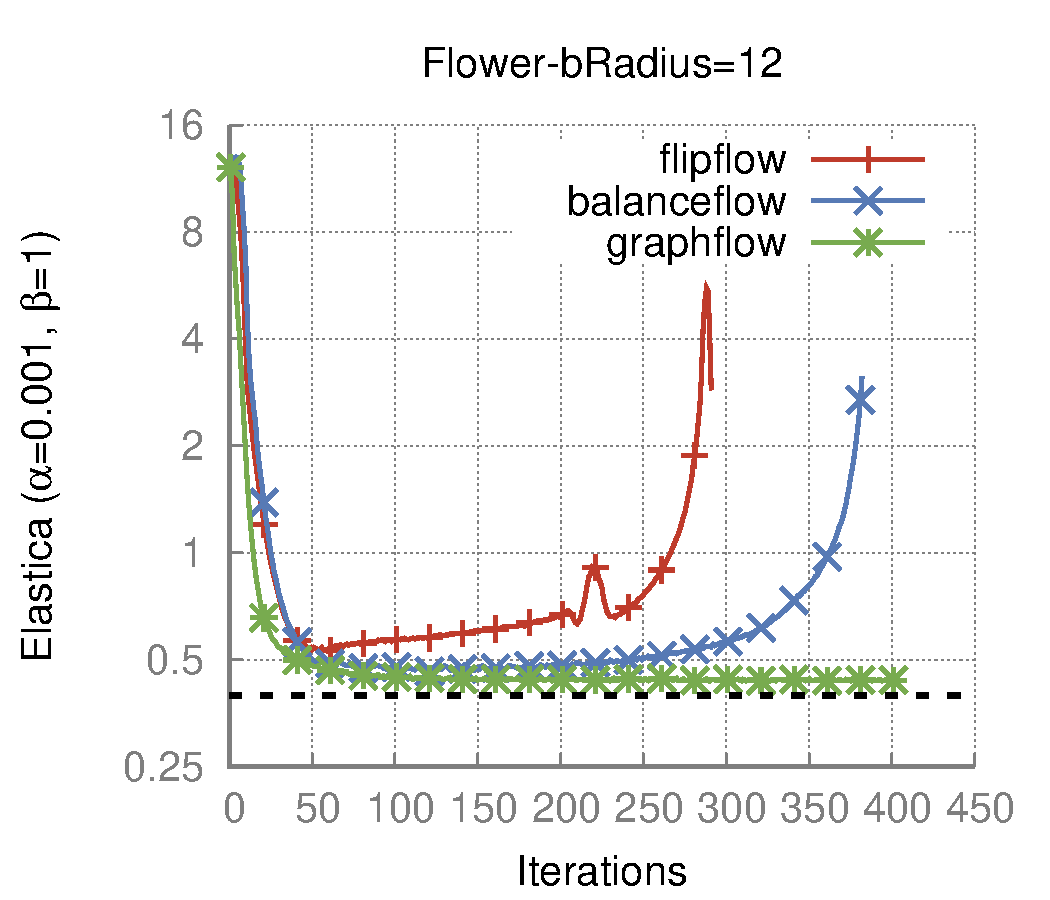
\includegraphics[scale=0.4]{figures/chapter9/free-elastica/plots/iteration/radius_choice/len_pen_0.001/radius-12/flower.pdf}
\end{tabular}
\caption{Digital Elastica value evolution per iteration of the Radius-choice experiment for the free Elastica.}
\label{fig:plots-free-elastica-radius-choice}
\end{figure}


\section{Constrained Elastica}

The constrained Elastica problem consists in to find the shape of minimum digital Elastica that respects some set of constraints. We realized experiments with two different set of constraints. In the first, we impose that a set of pixels in the digital boundary of the initial shape must persist in the final shape. In the second, we evolve a curve which the endpoints are fixed. 

For the constrained Elastica, only LocalSearch and GraphFlow were evaluated. We believe that both FlipFlow and BalanceFlow can be modified to evolve the constrained Elastica, but such modifications were not implemented in this thesis.~\cref{tab:constrained-elastica-parameters-summary} lists the parameters' used in the experiments and~\cref{tab:rtime-constrained-elastica-general} the running time of Exp-$\alpha$ experiment.

We remark that for every experiment in this section the grid step is set to $h=1.0$, i.e., the Euclidean and digital radius are the same. Differently from the previous section where all the shapes had a closed parametric formula, some of the tested shapes in this section are ad-hoc and a decision about the grid step in this case becomes arbitrary.

\subsection{Discussion}

Differently from LocalSearch, the GraphFlow model encounters some difficult to evolve both Curve-1 and Curve-2, as illustrated in~\cref{fig:results-constrained-elastica-general}. We recall that the LS model employs a more heterogeneous neighborhood than GF. The probe set of GF is created by applying erosions and dilations in the initial shape, which promotes quite rough transformations, i.e., they do not preserve any part of the contour. We believe that by refining the neighborhood, possibly a random one, we could obtain better results for the GraphFlow. Besides that, the GF evolves the Flower instances, though it stops at a shape of higher digital Elastica value than LS.

In~\cref{fig:results-constrained-elastica-radius} displays the results of experiment Exp-$bRadius$ in which the models are executed with different values for the radius of the estimation disk. As expected, a larger radius can estimate a large range of curvature values and it is particular important in the case where $\alpha=0.0002$. In this case the shape tends to grow and the estimator should be precise enough to identify small variations in curvature. Otherwise, the shape prematurely stops to evolve. Nonetheless, a radius that is too large (see~\cref{fig:constrained-elastica-underlying-curve-shapes}) may not be appropriated, and the curves do not evolve as expected.


\begin{table}
\centering
\begin{tabular}{|c|c|c|c|c|c|c|c|c|c|}
\cline{8-10}
\multicolumn{7}{c|}{} & LS & \multicolumn{2}{|c|}{GF}\\
\hline
Experiment & $maxIt$ & $vRadius$ & $bRadius$ & $h$ & $\alpha$ & $\beta$  & $nc$ & $a$ & $ob$ \\
\hline
\multirow{2}{*}{Exp-$\alpha$} & \multirow{2}{*}{$400$} & \multirow{2}{*}{$15$} & \multirow{2}{*}{$15$} & \multirow{2}{*}{$1.0$} & $0.002$ & \multirow{2}{*}{$1$}  & \multirow{2}{*}{$4$} & \multirow{2}{*}{$1$} & \multirow{2}{*}{$2$} \\
& & & & & $0.0002$ & & &\\
\hline
\multirow{2}{*}{Exp-$bRadius$} & \multirow{2}{*}{$400$} & $7$ & $7$ & \multirow{2}{*}{$1.0$} & \multirow{2}{*}{$0.0002$} & \multirow{2}{*}{$1$}  & \multirow{2}{*}{$4$} & \multirow{2}{*}{$1$} & \multirow{2}{*}{$2$} \\
& & $50$ & $50$ & & & & &\\
\hline
\end{tabular}
\caption{Parameter settings for the constrained Elastica experiments. The headers LS,GF identifies parameters that are exclusive for the LocalSearch and GraphFlow models, respectively.}
\label{tab:constrained-elastica-parameters-summary}
\end{table}

\begin{figure}
\center
\subfloat[Curve-1]{
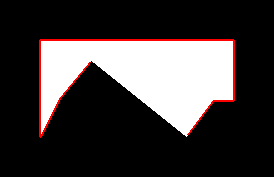
\includegraphics[scale=0.5]{figures/chapter9/constrained-elastica/curve-2/composite-fixed-pixels.png}
}
\subfloat[Curve-2]{
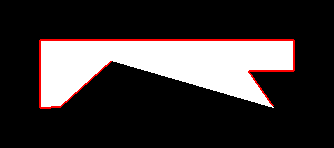
\includegraphics[scale=0.5]{figures/chapter9/constrained-elastica/curve-3/composite-fixed-pixels.png}
}
\subfloat[Too large radius]{
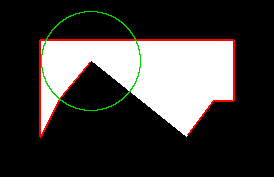
\includegraphics[scale=0.5]{figures/chapter9/constrained-elastica/curve-2/too-big-radius.png}
}
\caption{The underlying shapes of Curve-1 and Curve-2 for constrained Elastica experiments are shown in figures (a) and (b). Pixels in red are forced to persist in the solution. In figure (c), an example of a too large radius value $(50)$.}
\label{fig:constrained-elastica-underlying-curve-shapes}
\end{figure}


\begin{figure}
\center
\begin{tabular}{cccc}
\multicolumn{2}{c}{LocalSearch} & \multicolumn{2}{c}{GraphFlow}\\
$\alpha=0.002$ & $\alpha=0.0002$ & $\alpha=0.002$ & $\alpha=0.0002$\\
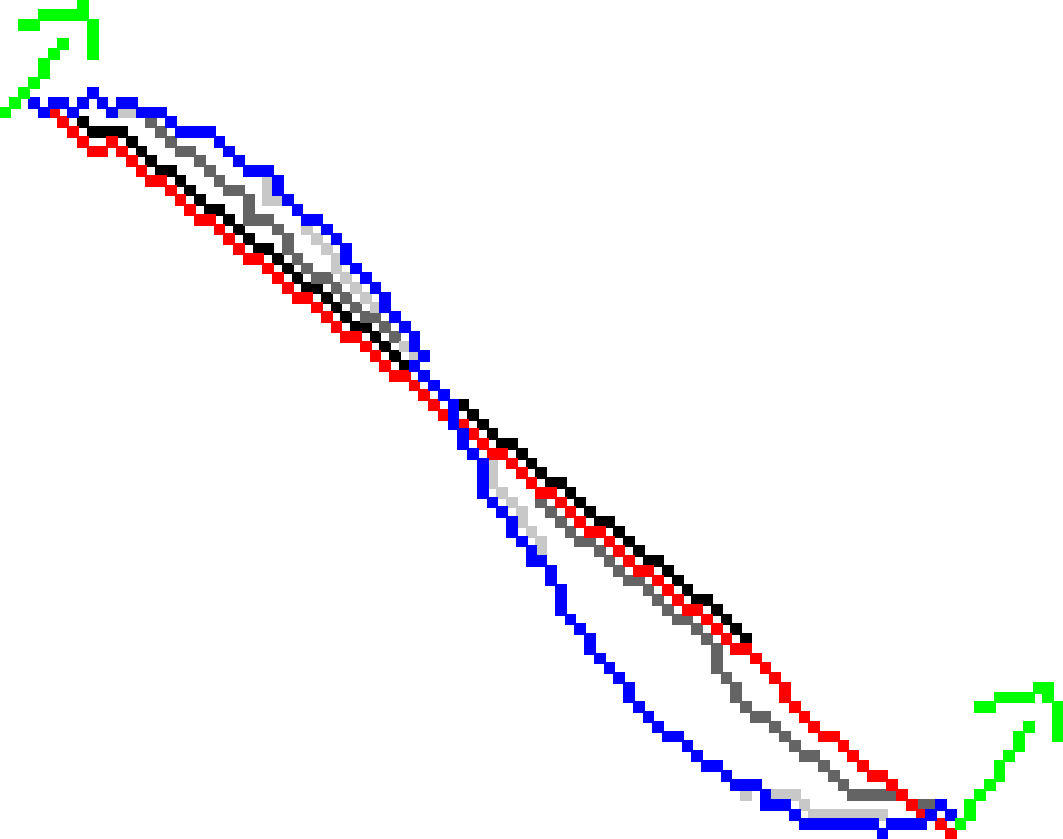
\includegraphics[scale=0.2]{figures/chapter9/constrained-elastica/localsearch/curve-2/len_pen-0.002/radius-15/nc-4/h1.0/summary.pdf} &
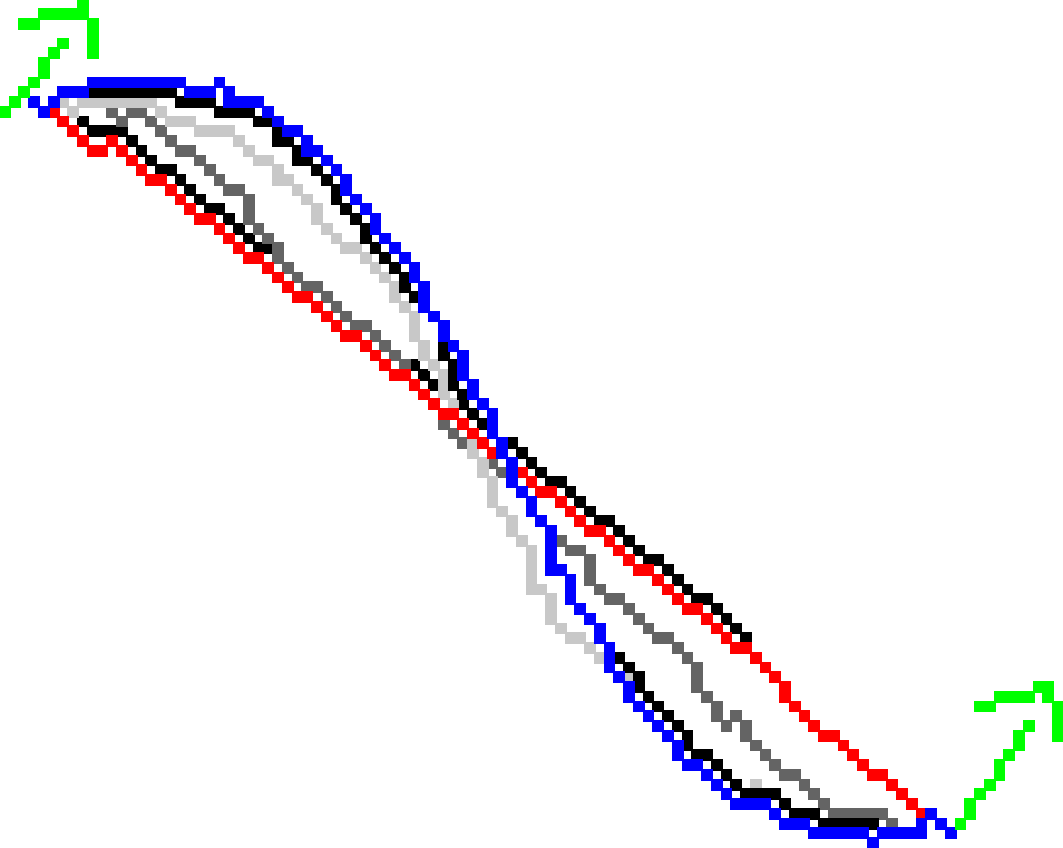
\includegraphics[scale=0.2]{figures/chapter9/constrained-elastica/localsearch/curve-2/len_pen-0.0002/radius-15/nc-4/h1.0/summary.pdf} &
\includegraphics[scale=0.25]{figures/chapter9/constrained-elastica/graphflow/curve-2/len_pen-0.002/radius-15/N-1/h1.0/summary.pdf} &
\includegraphics[scale=0.25]{figures/chapter9/constrained-elastica/graphflow/curve-2/len_pen-0.0002/radius-15/N-1/h1.0/summary.pdf}\\
\includegraphics[scale=0.2]{figures/chapter9/constrained-elastica/localsearch/curve-3/len_pen-0.002/radius-15/nc-4/h1.0/summary.pdf} &
\includegraphics[scale=0.2]{figures/chapter9/constrained-elastica/localsearch/curve-3/len_pen-0.0002/radius-15/nc-4/h1.0/summary.pdf} &
\includegraphics[scale=0.25]{figures/chapter9/constrained-elastica/graphflow/curve-3/len_pen-0.002/radius-15/N-1/h1.0/summary.pdf} &
\includegraphics[scale=0.25]{figures/chapter9/constrained-elastica/graphflow/curve-3/len_pen-0.0002/radius-15/N-1/h1.0/summary.pdf}\\
\includegraphics[scale=0.2]{figures/chapter9/constrained-elastica/localsearch/flower-1/len_pen-0.002/radius-15/nc-4/h1.0/summary.pdf} &
\includegraphics[scale=0.2]{figures/chapter9/constrained-elastica/localsearch/flower-1/len_pen-0.0002/radius-15/nc-4/h1.0/summary.pdf} &
\includegraphics[scale=0.25]{figures/chapter9/constrained-elastica/graphflow/flower-1/len_pen-0.002/radius-15/N-1/h1.0/summary.pdf} &
\includegraphics[scale=0.25]{figures/chapter9/constrained-elastica/graphflow/flower-1/len_pen-0.0002/radius-15/N-1/h1.0/summary.pdf}\\
\includegraphics[scale=0.2]{figures/chapter9/constrained-elastica/localsearch/flower-2/len_pen-0.002/radius-15/nc-4/h1.0/summary.pdf} &
\includegraphics[scale=0.2]{figures/chapter9/constrained-elastica/localsearch/flower-2/len_pen-0.0002/radius-15/nc-4/h1.0/summary.pdf} &
\includegraphics[scale=0.25]{figures/chapter9/constrained-elastica/graphflow/flower-2/len_pen-0.002/radius-15/N-1/h1.0/summary.pdf} &
\includegraphics[scale=0.25]{figures/chapter9/constrained-elastica/graphflow/flower-2/len_pen-0.0002/radius-15/N-1/h1.0/summary.pdf}\\
\end{tabular}
\caption{Results of Exp-$\alpha$ for the constrained Elastica. Initial contour is colored in red and final contour is colored in blue. The green pixels indicates pixels forced to persist in the final contour, or a forced orientation. Curves are drawn every $10$ iterations.}
\label{fig:results-constrained-elastica-general}
\end{figure}

\begin{figure}
\center
\begin{tabular}{cccc}
\multicolumn{2}{c}{LocalSearch} & \multicolumn{2}{c}{GraphFlow}\\
$r=7$ & $r=50$ & $r=7$ & $r=50$\\

\includegraphics[scale=0.2]{figures/chapter9/constrained-elastica/localsearch/curve-2/len_pen-0.0002/radius-7/nc-4/h1.0/summary.pdf} &
\includegraphics[scale=0.2]{figures/chapter9/constrained-elastica/localsearch/curve-2/len_pen-0.0002/radius-50/nc-4/h1.0/summary.pdf} &
\includegraphics[scale=0.2]{figures/chapter9/constrained-elastica/graphflow/curve-2/len_pen-0.0002/radius-7/N-1/h1.0/summary.pdf} &
\includegraphics[scale=0.2]{figures/chapter9/constrained-elastica/graphflow/curve-2/len_pen-0.0002/radius-50/N-1/h1.0/summary.pdf}\\

\includegraphics[scale=0.2]{figures/chapter9/constrained-elastica/localsearch/curve-3/len_pen-0.0002/radius-7/nc-4/h1.0/summary.pdf} &
\includegraphics[scale=0.2]{figures/chapter9/constrained-elastica/localsearch/curve-3/len_pen-0.0002/radius-50/nc-4/h1.0/summary.pdf} &
\includegraphics[scale=0.2]{figures/chapter9/constrained-elastica/graphflow/curve-3/len_pen-0.0002/radius-7/N-1/h1.0/summary.pdf} &
\includegraphics[scale=0.2]{figures/chapter9/constrained-elastica/graphflow/curve-3/len_pen-0.0002/radius-50/N-1/h1.0/summary.pdf}\\

\includegraphics[scale=0.2]{figures/chapter9/constrained-elastica/localsearch/flower-1/len_pen-0.0002/radius-7/nc-4/h1.0/summary.pdf} &
\includegraphics[scale=0.2]{figures/chapter9/constrained-elastica/localsearch/flower-1/len_pen-0.0002/radius-50/nc-4/h1.0/summary.pdf} &
\includegraphics[scale=0.2]{figures/chapter9/constrained-elastica/graphflow/flower-1/len_pen-0.0002/radius-7/N-1/h1.0/summary.pdf} &
\includegraphics[scale=0.2]{figures/chapter9/constrained-elastica/graphflow/flower-1/len_pen-0.0002/radius-50/N-1/h1.0/summary.pdf}\\

\includegraphics[scale=0.2]{figures/chapter9/constrained-elastica/localsearch/flower-2/len_pen-0.0002/radius-7/nc-4/h1.0/summary.pdf} &
\includegraphics[scale=0.2]{figures/chapter9/constrained-elastica/localsearch/flower-2/len_pen-0.0002/radius-50/nc-4/h1.0/summary.pdf} &
\includegraphics[scale=0.2]{figures/chapter9/constrained-elastica/graphflow/flower-2/len_pen-0.0002/radius-7/N-1/h1.0/summary.pdf} &
\includegraphics[scale=0.2]{figures/chapter9/constrained-elastica/graphflow/flower-2/len_pen-0.0002/radius-50/N-1/h1.0/summary.pdf}\\


\end{tabular}
\caption{Results of Exp-$bRadius$ for the constrained Elastica. Initial contour is colored in red and final contour is colored in blue. The green pixels indicates pixels forced to persist in the final contour, or a forced orientation. Curves are drawn every $10$ iterations.}
\label{fig:results-constrained-elastica-radius}
\end{figure}


\begin{figure}
\center
\captionsetup{type=table}
\begin{tabular}{|l|c|c|c|c|c|}
\hline
& Pixels (initial shape) & LocalSearch & GraphFlow \\
\hline
Curve-1 & 12306 & 4.7s/it & 1s/it\\
Curve-2 & 11527 & 6.2s/it & 1s/it\\
Flower-1  & 7481 & 4.5s/it & 0.3s/it \\
Flower-2 & 7481 & 2.5s/it & 0.21s/it\\
\hline
\end{tabular}
\caption{Running time and input size of the Exp-$\alpha$ experiment for the constrained Elastica. The pixels columns is with respect the number of pixels in the shape. In the case of the curves, it is with respect the underlying shapes of~\cref{fig:constrained-elastica-underlying-curve-shapes}}
\label{tab:rtime-constrained-elastica-general} 
\end{figure}

%The parameters used in the comparison are listed in table~\cref{} and the running times in table~\cref{}. The results are displayed in figures~\cref{} and~\cref{}, one for each value of $\alpha$. 

\section{Image segmentation}

The FlipFlow,BalanceFlow and GraphFlow can be extended to do image segmentation. In this section we show the results of several experiments that illustrates the influence of each of the the weights parameters (length,curvature,data) and the radius of the estimation ball in the produced segmentation. At the last section we compare our results with the Schoenemann linear curvature regularization (SLCR) \cite{schoenemann09linear}. 

All three models (FF,BF,GF) need a initial segmentation as input. This segmentation is given by a single iteration of the Grabcut algorithm.~\cref{tab:image-segmentation-parameters-summary} lists the parameters configuration for each experiment and~\cref{tab:rtime-image-segmentation-general} summarizes their running times. 

The experiments are divided in two sections. In the first, we study the influence of each parameter in the produced segmentation and in the second we compare our results with those produced by SLCR. For the same reason described in the previous section, the grid step in all experiments is set to $h=1.0$.


\begin{table}
\centering
\begin{tabular}{|c|c|c|c|c|c|c|c|c|c|c|c|c|}
\cline{8-13}
\multicolumn{7}{c|}{} & \multicolumn{2}{|c|}{FF,BF} & \multicolumn{4}{|c|}{GF}\\
\hline
Experiment & $maxIt$ & $vRadius$ & $bRadius$ & $h$ & $\alpha$ & $\beta$  & $\gamma$ & $d$ & $a$ & $ob$ & $\lambda_r$ & $\lambda_b$ \\
\hline
\multirow{3}{*}{Exp-$\alpha$} & \multirow{3}{*}{$200$} & \multirow{3}{*}{$7$} & \multirow{3}{*}{$7$} & \multirow{3}{*}{$1.0$} & $0$ & \multirow{3}{*}{$0$} & \multirow{3}{*}{$1$} & \multirow{3}{*}{$0$} & \multirow{3}{*}{$2$} & \multirow{3}{*}{$2$} & \multirow{3}{*}{$1$} & \multirow{3}{*}{$0$} \\
&  & & & & $0.5$ & & & & & & &\\
&  & & & & $3.0$ & & & & & & &\\
\hline
\multirow{3}{*}{Exp-$\beta$} & \multirow{3}{*}{$200$} & \multirow{3}{*}{$7$} & \multirow{3}{*}{$7$} & \multirow{3}{*}{$1.0$} & \multirow{3}{*}{$0$} & $0.1$ & \multirow{3}{*}{$1$} & \multirow{3}{*}{$0$} & \multirow{3}{*}{$2$} & \multirow{3}{*}{$2$} & \multirow{3}{*}{$1$} & \multirow{3}{*}{$1$} \\
&  & & & & & $1$ & & & & & &\\
&  & & & & & $2$ & & & & & &\\
\hline
\multirow{3}{*}{Exp-$\gamma$} & \multirow{3}{*}{$200$} & \multirow{3}{*}{$7$} & \multirow{3}{*}{$7$} & \multirow{3}{*}{$1.0$} & \multirow{3}{*}{$0$} & \multirow{3}{*}{$1$} & $1$ & \multirow{3}{*}{$0$} & \multirow{3}{*}{$2$} & \multirow{3}{*}{$2$} & $1$ & $1$ \\
&  & & & & & & $2$ & & & & $2$ & $2$\\
&  & & & & & & $5$ & & & & $5$ & $5$\\
\hline
\multirow{3}{*}{Exp-$rbRadius$} & \multirow{3}{*}{$200$} & $3$ & $3$ & \multirow{3}{*}{$1.0$} &  \multirow{3}{*}{$0$} & \multirow{3}{*}{$3$} & \multirow{3}{*}{$1$} & \multirow{3}{*}{$0$} & \multirow{3}{*}{$2$} & \multirow{3}{*}{$2$} & \multirow{3}{*}{$1$} & \multirow{3}{*}{$1$} \\
&  & $7$ & $7$ & & & & & & & & & \\
&  & $12$ & $12$ & & & & & & & & & \\
\hline
\end{tabular}
\caption{Parameter settings for the image segmentation experiments. The headers FF,BF,GF identifies parameters that are exclusive of FlipFlow, BalanceFlow and GraphFlow models, respectively.}
\label{tab:image-segmentation-parameters-summary}
\end{table}


\begin{table}
\centering
\begin{tabular}{|c|c|c|c|c|c|c|c|c|c|c|c|c|}
\hline
\multicolumn{13}{|c|}{Exp-Comparison}\\
\hline
Model & $maxIt$ & $vRadius$ & $bRadius$ & $h$ & $\alpha$ & $\beta (\lambda)$  & $\gamma$ & $d$ & $a$ & $ob$ & $\lambda_r$ & $\lambda_b$ \\
\hline
FF,BF & $200$ & $7$ & $7$ & $1.0$ & $0.5$ & $1.0$ & $1.0$ & $0$ & - & - & - & -\\
\hline
GF & $200$ & $7$ & $7$ & $1.0$ & $0.0002$ & $1.0$ & - & - & $2$ & $2$ & $3$ & $3$\\
\hline
SCLR & - & - & - & - & - & $2.0$ & $1.0$ & - & - & - & - & -\\
\hline
\end{tabular}
\caption{Parameter settings for the comparison experiments. The $\beta$ parameter in FF,BF,GF corresponds to the $\lambda$ parameter in SCLR.}
\label{tab:image-segmentation-comparison-summary}
\end{table}

\begin{figure}
\center
\captionsetup{type=table}
\begin{tabular}{|c|c|c|c|}
\hline
\multicolumn{4}{|c|}{Exp-Comparison Running time}\\
\hline
Model & Minimum & Maximum & Average \\
\hline
FlipFlow & 60s & 297s & 156s\\
BalanceFlow & 37s & 184s & 93.7s\\
GraphFlow & 11s & 150s & 75s\\
SLCR & 2.87min & 52.24min & 18.4min\\
\hline
\end{tabular}
\caption{Running time and input size of Exp-$bRadius$ for the image segmentation problem and $bRadius=7$.}
\label{tab:rtime-image-segmentation-general} 
\end{figure}

\subsection{Parameters influence}
The models offer parameters to control the relative weight of length $(\alpha)$, curvature $(\beta)$ and data ($\gamma,\lambda _r, \lambda _b$). We recall that FF and BF accept a single regional parameter $\gamma$ for data, while GF accepts $\lambda _r$ to ponderate a regional term and $\lambda _b$ to weight a boundary term. The Grabcut input and its result are shown in~\cref{fig:grabcut-input-image-segmentation}. The experiment results are displayed in~\cref{fig:exp-alpha-image-segmentation,fig:exp-beta-image-segmentation,fig:exp-gamma-image-segmentation,fig:exp-radius-image-segmentation}. 

The FlipFlow and BalanceFlow present similar results for all experiments, as expected. The Exp-$\alpha$ experiment regularizes only length, and we can observe that the segmentations produced by all three models tend to be staircased. We remark that in the GF model, length penalization is not present in the cost function of the candidate graph, but only in the validation function. In particular, we need  a $a$-probe set with $a>0$ to have length penalization an influence in the produced segmentation.

In experiment Exp-$\beta$ we vary the squared curvature weigth coefficient. We observe in~\cref{fig:exp-beta-image-segmentation} that the produced segmentation smooths out for increasing values of $\beta$. We recall that the shrink/growing behaviour in the GF is controlled by the value of $\alpha$. The FF, and BF grow in concavities, but unless a local optimum is found, it tends to shrink.

The models' response for the variation of data term is shown in~\cref{fig:exp-gamma-image-segmentation}. A higher value of $\gamma$ tends to produce results similar to the initial segmentation given by Grabcut, i.e., with almost no length or curvature regularization.

Finally, Exp-$bRadius$ illustrates how the choice of the estimation ball radius influences the segmentation. In~\cref{fig:exp-radius-image-segmentation} we observe that a small radius results in contours with sharp changes of angle (first row), a consequence of the limited number of different estimations that can be given by a ball of small radius. As the radius increase, a richer variation of estimations is possible, and we have smoother contours (second-row). However, a big radius may omit important details of the object, as the coala's ears in the last row of~\cref{fig:exp-radius-image-segmentation}. That suggests that a multiradius approach may deliver improved segmentations.


\begin{figure}
\centering
\begin{tabular}{cc}
\includegraphics[scale=0.4]{figures/chapter9/segmentation/seeds.png} &
\includegraphics[scale=0.4]{figures/chapter9/segmentation/gc-seg.png}
\end{tabular}
\caption{Foreground (green) and background (blue) seeds are shown in the left and the resulting Grabcut segmentation int the right.}
\label{fig:grabcut-input-image-segmentation}
\end{figure}

\newcommand\expAlphaFF[2]{figures/chapter9/segmentation/exp-alpha/#1/h-1.0/dalpha-False/neigh-0/alpha-#2/beta-0.0/lb-1.0/lr-1.0/coala/corrected_seg.png}
\newcommand\expAlphaGF[2]{figures/chapter9/segmentation/exp-alpha/#1/h-1.0/dalpha-False/neigh-2/alpha-#2/beta-0.0/lb-0.0/lr-1.0/coala/corrected_seg.png}

\begin{figure}
\centering
\begin{tabular}{cccc}
& FlipFlow & BalanceFlow & GraphFlow\\
$\alpha=0.0$ & 
\figTable{0.4}{\expAlphaFF{flipseg}{0.0}} &
\figTable{0.4}{\expAlphaFF{balanceseg}{0.0}} &
\figTable{0.4}{\expAlphaGF{graphseg}{0.0}}\\[10em]

$\alpha=0.5$ & 
\figTable{0.4}{\expAlphaFF{flipseg}{0.5}} &
\figTable{0.4}{\expAlphaFF{balanceseg}{0.5}} &
\figTable{0.4}{\expAlphaGF{graphseg}{0.5}}\\[10em]

$\alpha=3.0$ & 
\figTable{0.4}{\expAlphaFF{flipseg}{3.0}} &
\figTable{0.4}{\expAlphaFF{balanceseg}{3.0}} &
\figTable{0.4}{\expAlphaGF{graphseg}{3.0}}
\end{tabular}
\caption{Exp-$\alpha$}
\label{fig:exp-alpha-image-segmentation}
\end{figure}

\newcommand\expBetaFF[2]{figures/chapter9/segmentation/exp-beta/#1/h-1.0/dalpha-False/neigh-0/alpha-0.0/beta-#2/lb-1.0/lr-1.0/coala/corrected_seg.png}
\newcommand\expBetaGF[2]{figures/chapter9/segmentation/exp-beta/#1/h-1.0/dalpha-False/neigh-2/alpha-0.0/beta-#2/lb-1.0/lr-1.0/coala/corrected_seg.png}

\begin{figure}
\begin{tabular}{cccc}
& FlipFlow & BalanceFlow & GraphFlow\\
$\beta=0.1$ & 
\figTable{0.4}{\expBetaFF{flipseg}{0.1}} &
\figTable{0.4}{\expBetaFF{balanceseg}{0.1}} &
\figTable{0.4}{\expBetaGF{graphseg}{0.1}}\\[10em]

$\beta=1.0$ & 
\figTable{0.4}{\expBetaFF{flipseg}{1.0}} &
\figTable{0.4}{\expBetaFF{balanceseg}{1.0}} &
\figTable{0.4}{\expBetaGF{graphseg}{1.0}}\\[10em]

$\beta=2.0$ & 
\figTable{0.4}{\expBetaFF{flipseg}{2.0}} &
\figTable{0.4}{\expBetaFF{balanceseg}{2.0}} &
\figTable{0.4}{\expBetaGF{graphseg}{2.0}}

\end{tabular}
\caption{Exp-$\beta$}
\label{fig:exp-beta-image-segmentation}
\end{figure}

\newcommand\expGamaFF[2]{figures/chapter9/segmentation/exp-gamma/#1/h-1.0/dalpha-False/neigh-0/alpha-0.0/beta-1.0/lb-#2/lr-#2/coala/corrected_seg.png}
\newcommand\expGamaGF[2]{figures/chapter9/segmentation/exp-gamma/#1/h-1.0/dalpha-False/neigh-2/alpha-0.0/beta-1.0/lb-#2/lr-#2/coala/corrected_seg.png}

\begin{figure}
\begin{tabular}{cccc}
& FlipFlow & BalanceFlow & GraphFlow\\
$\gamma =1.0$ & 
\figTable{0.4}{\expGamaFF{flipseg}{1.0}} &
\figTable{0.4}{\expGamaFF{balanceseg}{1.0}} &
\figTable{0.4}{\expGamaGF{graphseg}{1.0}}\\[10em]

$\gamma =2.0$ & 
\figTable{0.4}{\expGamaFF{flipseg}{2.0}} &
\figTable{0.4}{\expGamaFF{balanceseg}{2.0}} &
\figTable{0.4}{\expGamaGF{graphseg}{2.0}}\\[10em]

$\gamma =5.0$ & 
\figTable{0.4}{\expGamaFF{flipseg}{5.0}} &
\figTable{0.4}{\expGamaFF{balanceseg}{5.0}} &
\figTable{0.4}{\expGamaGF{graphseg}{5.0}}

\end{tabular}
\caption{Exp-$\gamma$}
\label{fig:exp-gamma-image-segmentation}
\end{figure}


\newcommand\expRadiusFF[2]{figures/chapter9/segmentation/exp-radius/#1/h-1.0/alpha-0.0/beta-3.0/gamma-1.0/radius-#2/corrected-seg.png}
\newcommand\expRadiusGF[2]{figures/chapter9/segmentation/exp-radius/#1/h-1.0/alpha-0.0/beta-3.0/gamma-1.0/radius-#2/corrected-seg.png}

\begin{figure}
\begin{tabular}{cccc}
& FlipFlow & BalanceFlow & GraphFlow\\
$r=3$ & 
\figTable{0.4}{\expRadiusFF{flipseg}{3}} &
\figTable{0.4}{\expRadiusFF{balanceseg}{3}} &
\figTable{0.4}{\expRadiusGF{graphseg}{3}}\\[10em]

$r=7$ & 
\figTable{0.4}{\expRadiusFF{flipseg}{7}} &
\figTable{0.4}{\expRadiusFF{balanceseg}{7}} &
\figTable{0.4}{\expRadiusGF{graphseg}{7}}\\[10em]

$r=12$ & 
\figTable{0.4}{\expRadiusFF{flipseg}{12}} &
\figTable{0.4}{\expRadiusFF{balanceseg}{12}} &
\figTable{0.4}{\expRadiusGF{graphseg}{12}}
\end{tabular}
\caption{Exp-$bRadius$}
\label{fig:exp-radius-image-segmentation}
\end{figure}


\subsection{Comparison}

In~\cref{fig:exp-comparison-image-segmentation-1,fig:exp-comparison-image-segmentation-2,fig:exp-comparison-image-segmentation-3,fig:exp-comparison-image-segmentation-4} we show the segmentation results of several images for the three models developed in this thesis and the SLCR model. We opt to set the same parameters in all instances, although a better segmentation could be obtained by setting them separately.

The curvature regularization in the FF,BF models are well perceived in the airplane, camel and man-in-white pictures, but those models are not able to correctly segment the brown-snake in~\cref{fig:exp-comparison-image-segmentation-4}. They also have a hard time to segment the birds in~\cref{fig:exp-comparison-image-segmentation-2} due to the object large curvature interval jointly with the single radius approach adopted in this experiments. Nonetheless, they correctly segmented the green-snake in~\cref{fig:exp-comparison-image-segmentation-3} while the Grabcut return three disconnected components.

For the chosen parameters the GraphFlow did not evolved the Grabcut segmentationn to much, except for the brown-snake in~\cref{fig:exp-comparison-image-segmentation-4}, which GF and SLCR presented the best segmentation. However, the GF has the best lowest running time among the four models.

The SLCR tends to oversegment, notably in the man-in-white and the camel pictures. We observe that the contours present sharp turns due to the low precision of the curvature estimator. The precision could be improved by increasing the pixels connectivity (set to $8$), but is likely to follow a increase in running time, which is already the highest between the models tested.





\newcommand\segComparisonGF[2]{figures/chapter9/segmentation/comparison/#1/#2/alpha-0.0002/beta-1.0/gamma-3.0/radius-7}
\newcommand\segComparisonFF[2]{figures/chapter9/segmentation/comparison/#1/#2/alpha-0.5/beta-1.0/gamma-3.0/radius-7}
\newcommand\segComparisonScho[2]{figures/chapter9/segmentation/comparison/#1/lambda-2.0/gamma-1.0/#2}

\newcommand\compTable[5]{
	\begin{figure}
	\center
	\begin{tabular}{m{0.25cm}ccc}
	\rotatebox{90}{GrabCut} & 
	\figTable{0.32}{\segComparisonFF{flipseg}{#1}/gc-seg.png} & 
	\figTable{0.32}{\segComparisonFF{flipseg}{#2}/gc-seg.png} & 
	\figTable{0.32}{\segComparisonFF{flipseg}{#3}/gc-seg.png} \\[6em]
	
	\rotatebox{90}{SCLR} & 
	\figTable{0.32}{\segComparisonScho{schoenemann}{#1}/#1.png} & 
	\figTable{0.32}{\segComparisonScho{schoenemann}{#2}/#2.png} & 
	\figTable{0.32}{\segComparisonScho{schoenemann}{#3}/#3.png}\\[6em]
	
	\rotatebox{90}{FlipFlow} & 
	\figTable{0.32}{\segComparisonFF{flipseg}{#1}/corrected-seg.png} & 
	\figTable{0.32}{\segComparisonFF{flipseg}{#2}/corrected-seg.png} & 
	\figTable{0.32}{\segComparisonFF{flipseg}{#3}/corrected-seg.png} \\[6em]
	
	\rotatebox{90}{BalanceFlow} & 
	\figTable{0.32}{\segComparisonFF{balanceseg}{#1}/corrected-seg.png} & 
	\figTable{0.32}{\segComparisonFF{balanceseg}{#2}/corrected-seg.png} & 
	\figTable{0.32}{\segComparisonFF{balanceseg}{#3}/corrected-seg.png}\\[6em]
	
	\rotatebox{90}{GraphFlow} & 
	\figTable{0.32}{\segComparisonGF{graphseg}{#1}/corrected-seg.png} & 
	\figTable{0.32}{\segComparisonGF{graphseg}{#2}/corrected-seg.png} & 
	\figTable{0.32}{\segComparisonGF{graphseg}{#3}/corrected-seg.png}
	\end{tabular}
	\caption{#4}
	\label{#5}
	\end{figure}
}


\compTable{airplane}{kite-surf}{mans-music}{Comparison 1}{fig:exp-comparison-image-segmentation-1}
\compTable{birds}{brown-snake}{tiger}{Comparison 2}{fig:exp-comparison-image-segmentation-2}
\compTable{camel}{green-snake}{peacock}{Comparison 3}{fig:exp-comparison-image-segmentation-3}
%\compTable{long-snake}{mushroom}{statues}{Comparison 4}{fig:exp-comparison-image-segmentation-4}


\afterpage{%
    \clearpage% Flush earlier floats (otherwise order might not be correct)
    \thispagestyle{empty}% empty page style (?)
    \begin{landscape}% Landscape page

	\begin{figure}
	\center
	\begin{tabular}{ccccc}
	GrabCut & SLCR & FlipFlow & BalanceFlow & GraphFlow\\
	\figTable{0.32}{\segComparisonFF{flipseg}{long-snake}/gc-seg.png} & 
	\figTable{0.32}{\segComparisonScho{schoenemann}{long-snake}/long-snake.png} & 
	\figTable{0.32}{\segComparisonFF{flipseg}{long-snake}/corrected-seg.png} & 		
	\figTable{0.32}{\segComparisonFF{balanceseg}{long-snake}/corrected-seg.png} & 			
	\figTable{0.32}{\segComparisonGF{graphseg}{long-snake}/corrected-seg.png} \\[10em]	
	
	\figTable{0.32}{\segComparisonFF{flipseg}{statues}/gc-seg.png} & 
	\figTable{0.32}{\segComparisonScho{schoenemann}{statues}/statues.png} & 
	\figTable{0.32}{\segComparisonFF{flipseg}{statues}/corrected-seg.png} & 		
	\figTable{0.32}{\segComparisonFF{balanceseg}{statues}/corrected-seg.png} & 			
	\figTable{0.32}{\segComparisonGF{graphseg}{statues}/corrected-seg.png}
	
	
	\end{tabular}
	\caption{Comparison 4}
	\label{fig:exp-comparison-image-segmentation-4}
	\end{figure}

    \end{landscape}
    \clearpage% Flush page
}



\section{Conclusion}

All the four models described in this thesis can be used to produce shapes of lower digital Elastica. Moreover, the FlipFlow,BalanceFlow and GraphFlow can be extended to do image segmentation with curvature regularization. In particular, the GraphFlow is a straightforward extension of the standard Grabcut model, which originally does not implement geometric regularization, and presents lower running times than FF and BF. Finally, our models have shown to be competitive with the SLCR segmentation algorithm that employs curvature regularization.




